% Options for packages loaded elsewhere
\PassOptionsToPackage{unicode}{hyperref}
\PassOptionsToPackage{hyphens}{url}
%
\documentclass[
]{book}
\usepackage{lmodern}
\usepackage{amssymb,amsmath}
\usepackage{ifxetex,ifluatex}
\ifnum 0\ifxetex 1\fi\ifluatex 1\fi=0 % if pdftex
  \usepackage[T1]{fontenc}
  \usepackage[utf8]{inputenc}
  \usepackage{textcomp} % provide euro and other symbols
\else % if luatex or xetex
  \usepackage{unicode-math}
  \defaultfontfeatures{Scale=MatchLowercase}
  \defaultfontfeatures[\rmfamily]{Ligatures=TeX,Scale=1}
\fi
% Use upquote if available, for straight quotes in verbatim environments
\IfFileExists{upquote.sty}{\usepackage{upquote}}{}
\IfFileExists{microtype.sty}{% use microtype if available
  \usepackage[]{microtype}
  \UseMicrotypeSet[protrusion]{basicmath} % disable protrusion for tt fonts
}{}
\makeatletter
\@ifundefined{KOMAClassName}{% if non-KOMA class
  \IfFileExists{parskip.sty}{%
    \usepackage{parskip}
  }{% else
    \setlength{\parindent}{0pt}
    \setlength{\parskip}{6pt plus 2pt minus 1pt}}
}{% if KOMA class
  \KOMAoptions{parskip=half}}
\makeatother
\usepackage{xcolor}
\IfFileExists{xurl.sty}{\usepackage{xurl}}{} % add URL line breaks if available
\IfFileExists{bookmark.sty}{\usepackage{bookmark}}{\usepackage{hyperref}}
\hypersetup{
  pdftitle={Bayesian Modeling Using Stan},
  pdfauthor={Jim Albert},
  hidelinks,
  pdfcreator={LaTeX via pandoc}}
\urlstyle{same} % disable monospaced font for URLs
\usepackage{color}
\usepackage{fancyvrb}
\newcommand{\VerbBar}{|}
\newcommand{\VERB}{\Verb[commandchars=\\\{\}]}
\DefineVerbatimEnvironment{Highlighting}{Verbatim}{commandchars=\\\{\}}
% Add ',fontsize=\small' for more characters per line
\usepackage{framed}
\definecolor{shadecolor}{RGB}{248,248,248}
\newenvironment{Shaded}{\begin{snugshade}}{\end{snugshade}}
\newcommand{\AlertTok}[1]{\textcolor[rgb]{0.94,0.16,0.16}{#1}}
\newcommand{\AnnotationTok}[1]{\textcolor[rgb]{0.56,0.35,0.01}{\textbf{\textit{#1}}}}
\newcommand{\AttributeTok}[1]{\textcolor[rgb]{0.77,0.63,0.00}{#1}}
\newcommand{\BaseNTok}[1]{\textcolor[rgb]{0.00,0.00,0.81}{#1}}
\newcommand{\BuiltInTok}[1]{#1}
\newcommand{\CharTok}[1]{\textcolor[rgb]{0.31,0.60,0.02}{#1}}
\newcommand{\CommentTok}[1]{\textcolor[rgb]{0.56,0.35,0.01}{\textit{#1}}}
\newcommand{\CommentVarTok}[1]{\textcolor[rgb]{0.56,0.35,0.01}{\textbf{\textit{#1}}}}
\newcommand{\ConstantTok}[1]{\textcolor[rgb]{0.00,0.00,0.00}{#1}}
\newcommand{\ControlFlowTok}[1]{\textcolor[rgb]{0.13,0.29,0.53}{\textbf{#1}}}
\newcommand{\DataTypeTok}[1]{\textcolor[rgb]{0.13,0.29,0.53}{#1}}
\newcommand{\DecValTok}[1]{\textcolor[rgb]{0.00,0.00,0.81}{#1}}
\newcommand{\DocumentationTok}[1]{\textcolor[rgb]{0.56,0.35,0.01}{\textbf{\textit{#1}}}}
\newcommand{\ErrorTok}[1]{\textcolor[rgb]{0.64,0.00,0.00}{\textbf{#1}}}
\newcommand{\ExtensionTok}[1]{#1}
\newcommand{\FloatTok}[1]{\textcolor[rgb]{0.00,0.00,0.81}{#1}}
\newcommand{\FunctionTok}[1]{\textcolor[rgb]{0.00,0.00,0.00}{#1}}
\newcommand{\ImportTok}[1]{#1}
\newcommand{\InformationTok}[1]{\textcolor[rgb]{0.56,0.35,0.01}{\textbf{\textit{#1}}}}
\newcommand{\KeywordTok}[1]{\textcolor[rgb]{0.13,0.29,0.53}{\textbf{#1}}}
\newcommand{\NormalTok}[1]{#1}
\newcommand{\OperatorTok}[1]{\textcolor[rgb]{0.81,0.36,0.00}{\textbf{#1}}}
\newcommand{\OtherTok}[1]{\textcolor[rgb]{0.56,0.35,0.01}{#1}}
\newcommand{\PreprocessorTok}[1]{\textcolor[rgb]{0.56,0.35,0.01}{\textit{#1}}}
\newcommand{\RegionMarkerTok}[1]{#1}
\newcommand{\SpecialCharTok}[1]{\textcolor[rgb]{0.00,0.00,0.00}{#1}}
\newcommand{\SpecialStringTok}[1]{\textcolor[rgb]{0.31,0.60,0.02}{#1}}
\newcommand{\StringTok}[1]{\textcolor[rgb]{0.31,0.60,0.02}{#1}}
\newcommand{\VariableTok}[1]{\textcolor[rgb]{0.00,0.00,0.00}{#1}}
\newcommand{\VerbatimStringTok}[1]{\textcolor[rgb]{0.31,0.60,0.02}{#1}}
\newcommand{\WarningTok}[1]{\textcolor[rgb]{0.56,0.35,0.01}{\textbf{\textit{#1}}}}
\usepackage{longtable,booktabs}
% Correct order of tables after \paragraph or \subparagraph
\usepackage{etoolbox}
\makeatletter
\patchcmd\longtable{\par}{\if@noskipsec\mbox{}\fi\par}{}{}
\makeatother
% Allow footnotes in longtable head/foot
\IfFileExists{footnotehyper.sty}{\usepackage{footnotehyper}}{\usepackage{footnote}}
\makesavenoteenv{longtable}
\usepackage{graphicx,grffile}
\makeatletter
\def\maxwidth{\ifdim\Gin@nat@width>\linewidth\linewidth\else\Gin@nat@width\fi}
\def\maxheight{\ifdim\Gin@nat@height>\textheight\textheight\else\Gin@nat@height\fi}
\makeatother
% Scale images if necessary, so that they will not overflow the page
% margins by default, and it is still possible to overwrite the defaults
% using explicit options in \includegraphics[width, height, ...]{}
\setkeys{Gin}{width=\maxwidth,height=\maxheight,keepaspectratio}
% Set default figure placement to htbp
\makeatletter
\def\fps@figure{htbp}
\makeatother
\setlength{\emergencystretch}{3em} % prevent overfull lines
\providecommand{\tightlist}{%
  \setlength{\itemsep}{0pt}\setlength{\parskip}{0pt}}
\setcounter{secnumdepth}{5}
\usepackage{booktabs}
\usepackage{amsthm}
\makeatletter
\def\thm@space@setup{%
  \thm@preskip=8pt plus 2pt minus 4pt
  \thm@postskip=\thm@preskip
}
\makeatother
\usepackage[]{natbib}
\bibliographystyle{apalike}

\title{Bayesian Modeling Using Stan}
\author{Jim Albert}
\date{2020-07-14}

\begin{document}
\maketitle

{
\setcounter{tocdepth}{1}
\tableofcontents
}
\hypertarget{introduction-to-the-brms-package}{%
\chapter{Introduction to the brms Package}\label{introduction-to-the-brms-package}}

In \textbf{Probability and Bayesian Modeling}, the JAGS software is illustrated to fit various Bayesian models by Markov Chain Monte Carlo (MCMC) methods. JAGS consists of a mix of conjugate, Gibbs sampling, and Metropolis algorithms. In recent years, Hamiltonian sampling and the associated Stan software are becoming popular in fitting Bayesian models by MCMC.

The purpose of this supplement is to illustrate Bayesian fitting of common models using the \texttt{brms} package which is a popular interface for the Stan software.

\hypertarget{installing-the-brms-package}{%
\section{\texorpdfstring{Installing the \texttt{brms} package}{Installing the brms package}}\label{installing-the-brms-package}}

Basic information about installing the \texttt{brms} package is available at \url{https://github.com/paul-buerkner/brms}

Since the package is an interface to the Stan software, a C++ compiler is required.

\hypertarget{one-bayesian-fitting-function-brm}{%
\section{\texorpdfstring{One Bayesian fitting function \texttt{brm()}}{One Bayesian fitting function brm()}}\label{one-bayesian-fitting-function-brm}}

One attractive feature of the \texttt{brms} package is that one function \texttt{brm()} can be used to fit all of the models described in \textbf{Probability and Bayesian Modeling}.

The basic function syntax of the \texttt{brm()} function is:

\begin{verbatim}
brm(model_description, 
    data = my_data, 
    family = the_family,
    prior = the_prior)
\end{verbatim}

where

\begin{itemize}
\tightlist
\item
  \texttt{model\_description} is the description of the regression model including any random effects similar to the notation used in the \texttt{glm()} and \texttt{glmer} functions
\item
  \texttt{my\_data} is the data frame containing the data
\item
  \texttt{family} is the sampling family (normal, binomial, Poisson, etc)
\item
  \texttt{prior} is the specification of the prior on the regression terms and the error standard deviation
\end{itemize}

The output of the \texttt{brm()} function is an object of class brmsfit that contains the posterior samples and other information about the model.

\begin{center}\rule{0.5\linewidth}{0.5pt}\end{center}

\hypertarget{binomial-modeling}{%
\chapter{Binomial Modeling}\label{binomial-modeling}}

\hypertarget{packages-for-example}{%
\section{Packages for example}\label{packages-for-example}}

\begin{Shaded}
\begin{Highlighting}[]
\KeywordTok{library}\NormalTok{(ProbBayes)}
\KeywordTok{library}\NormalTok{(brms)}
\KeywordTok{library}\NormalTok{(dplyr)}
\KeywordTok{library}\NormalTok{(ggplot2)}
\end{Highlighting}
\end{Shaded}

\hypertarget{example}{%
\section{Example}\label{example}}

Suppose a sample of \(n = 20\) college students are asked if they plan on wearing masks while attending class. Let \(p\) denote the proportion of all students who plan on wearing masks.

\hypertarget{prior-on-proportion}{%
\section{Prior on proportion}\label{prior-on-proportion}}

Suppose you believe that \(p = 0.40\) and you are 90 percent sure that \(p < 0.60\).

Use \texttt{beta.select()} from the \texttt{ProbBayes} package to find the shape parameters of the matching beta curve prior.

\begin{Shaded}
\begin{Highlighting}[]
\KeywordTok{beta.select}\NormalTok{(}\KeywordTok{list}\NormalTok{(}\DataTypeTok{x =} \FloatTok{0.4}\NormalTok{, }\DataTypeTok{p =} \FloatTok{0.5}\NormalTok{),}
            \KeywordTok{list}\NormalTok{(}\DataTypeTok{x =} \FloatTok{0.6}\NormalTok{, }\DataTypeTok{p =} \FloatTok{0.9}\NormalTok{))}
\end{Highlighting}
\end{Shaded}

\begin{verbatim}
## [1] 4.31 6.30
\end{verbatim}

A beta(4.31, 6.30) prior represents one's beliefs about the proportion \(p\).

\hypertarget{prior-on-the-logit-parameter}{%
\section{Prior on the logit parameter}\label{prior-on-the-logit-parameter}}

Since we will writing a model in terms of the logit function
\[
\theta = \log \left(\frac{p}{1-p}\right)
\]

We want to find a corresponding normal prior on \(\theta\).

A simple way of doing this is by simulation \ldots{}

\begin{enumerate}
\def\labelenumi{\arabic{enumi}.}
\tightlist
\item
  Simulate 1000 draws from the beta prior on \(p\).
\item
  Compute \(\theta\) on these simulated draws of \(p\).
\item
  Find the sample mean and standard deviation of these draws -- those will be estimates of the mean and standard deviation of the normal prior on \(\theta\).
\end{enumerate}

\begin{Shaded}
\begin{Highlighting}[]
\KeywordTok{set.seed}\NormalTok{(}\DecValTok{123}\NormalTok{)}
\NormalTok{p_sim <-}\StringTok{ }\KeywordTok{rbeta}\NormalTok{(}\DecValTok{1000}\NormalTok{, }\FloatTok{4.31}\NormalTok{, }\FloatTok{6.30}\NormalTok{)}
\NormalTok{theta_sim <-}\StringTok{ }\KeywordTok{log}\NormalTok{(p_sim }\OperatorTok{/}\StringTok{ }\NormalTok{(}\DecValTok{1} \OperatorTok{-}\StringTok{ }\NormalTok{p_sim))}
\KeywordTok{c}\NormalTok{(}\KeywordTok{mean}\NormalTok{(theta_sim), }\KeywordTok{sd}\NormalTok{(theta_sim))}
\end{Highlighting}
\end{Shaded}

\begin{verbatim}
## [1] -0.4000904  0.6540093
\end{verbatim}

The corresponding prior on the logit parameter \(\theta\) is assumed to be normal with mean \(-0.400\) and standard deviation \(0.654\).

\hypertarget{fitting-the-model}{%
\section{Fitting the model}\label{fitting-the-model}}

The model is \(y_1, ..., y_{20}\) are a random sample from a Bernoulli distribution with probability \(p\) where \(p\) has the logistic representation.

\[
\log \left(\frac{p}{1-p}\right) = \theta
\]

where \(\theta \sim N(-0.400, 0.654)\).

We put the twenty binary responses in a data frame.

\begin{Shaded}
\begin{Highlighting}[]
\NormalTok{bdata <-}\StringTok{ }\KeywordTok{data.frame}\NormalTok{(}\DataTypeTok{y =} \KeywordTok{c}\NormalTok{(}\DecValTok{1}\NormalTok{, }\DecValTok{0}\NormalTok{, }\DecValTok{1}\NormalTok{, }\DecValTok{0}\NormalTok{, }\DecValTok{0}\NormalTok{, }\DecValTok{0}\NormalTok{, }\DecValTok{1}\NormalTok{, }
\DecValTok{0}\NormalTok{, }\DecValTok{0}\NormalTok{, }\DecValTok{1}\NormalTok{, }\DecValTok{0}\NormalTok{, }\DecValTok{0}\NormalTok{, }\DecValTok{0}\NormalTok{, }\DecValTok{1}\NormalTok{, }\DecValTok{1}\NormalTok{, }\DecValTok{0}\NormalTok{, }\DecValTok{0}\NormalTok{, }\DecValTok{0}\NormalTok{, }\DecValTok{1}\NormalTok{, }\DecValTok{0}\NormalTok{))}
\end{Highlighting}
\end{Shaded}

We use the \texttt{brm()} function from the \texttt{brms} package to fit the model.

\begin{Shaded}
\begin{Highlighting}[]
\NormalTok{fit <-}\StringTok{ }\KeywordTok{brm}\NormalTok{(}\DataTypeTok{data =}\NormalTok{ bdata, }
            \DataTypeTok{family =}\NormalTok{ bernoulli,}
\NormalTok{            y  }\OperatorTok{~}\StringTok{ }\DecValTok{0} \OperatorTok{+}\StringTok{ }\NormalTok{Intercept,}
            \DataTypeTok{prior =} \KeywordTok{c}\NormalTok{(}\KeywordTok{prior}\NormalTok{(}\KeywordTok{normal}\NormalTok{(}\OperatorTok{-}\FloatTok{0.400}\NormalTok{, }\FloatTok{0.654}\NormalTok{), }
                           \DataTypeTok{coef =}\NormalTok{ Intercept)),}
            \DataTypeTok{iter =} \DecValTok{1000}\NormalTok{,}
            \DataTypeTok{refresh =} \DecValTok{0}\NormalTok{)}
\end{Highlighting}
\end{Shaded}

\begin{verbatim}
## Compiling Stan program...
\end{verbatim}

\begin{verbatim}
## Start sampling
\end{verbatim}

The \texttt{plot()} function will display a density plot and a trace plot of the intercept \(\theta\).

\begin{Shaded}
\begin{Highlighting}[]
\KeywordTok{plot}\NormalTok{(fit)}
\end{Highlighting}
\end{Shaded}

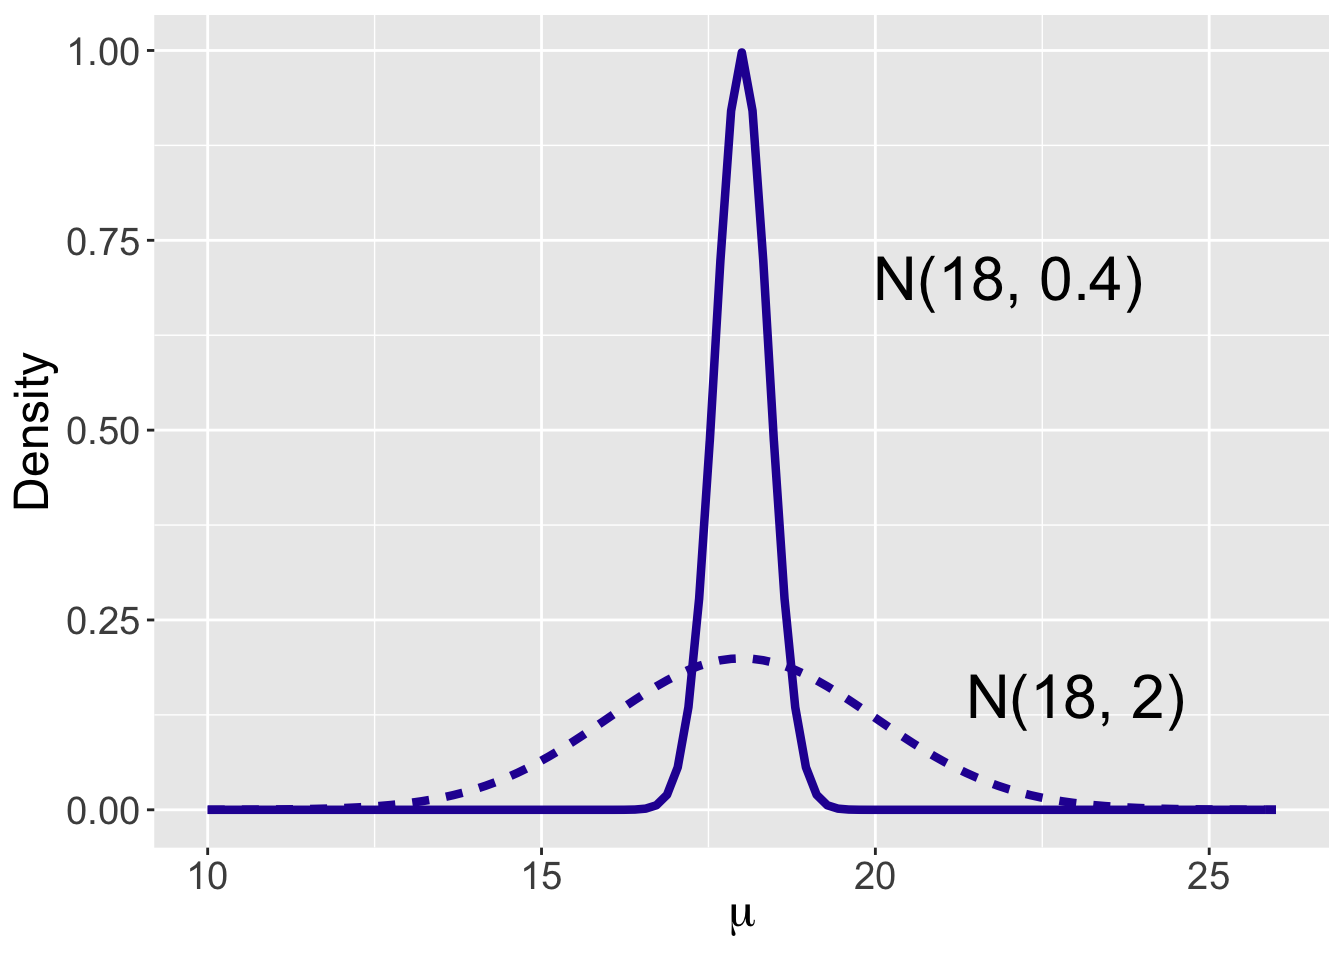
\includegraphics{bookdown-demo_files/figure-latex/unnamed-chunk-7-1.pdf}

The \texttt{summary()} function provides summary statistics for \(\theta\).

\begin{Shaded}
\begin{Highlighting}[]
\KeywordTok{summary}\NormalTok{(fit)}
\end{Highlighting}
\end{Shaded}

\begin{verbatim}
##  Family: bernoulli 
##   Links: mu = logit 
## Formula: y ~ 0 + Intercept 
##    Data: bdata (Number of observations: 20) 
## Samples: 4 chains, each with iter = 1000; warmup = 500; thin = 1;
##          total post-warmup samples = 2000
## 
## Population-Level Effects: 
##           Estimate Est.Error l-95% CI u-95% CI Rhat Bulk_ESS Tail_ESS
## Intercept    -0.56      0.39    -1.29     0.17 1.01      684     1111
## 
## Samples were drawn using sampling(NUTS). For each parameter, Bulk_ESS
## and Tail_ESS are effective sample size measures, and Rhat is the potential
## scale reduction factor on split chains (at convergence, Rhat = 1).
\end{verbatim}

The \texttt{posterior\_samples()} function will display the simulated draws of \(\theta\).

\begin{Shaded}
\begin{Highlighting}[]
\NormalTok{post <-}\StringTok{ }\KeywordTok{posterior_samples}\NormalTok{(fit)}
\KeywordTok{head}\NormalTok{(post)}
\end{Highlighting}
\end{Shaded}

\begin{verbatim}
##   b_Intercept      lp__
## 1  -0.3644459 -13.59560
## 2  -0.4101895 -13.54451
## 3  -0.5691616 -13.48236
## 4   0.3479299 -16.35609
## 5   0.5788761 -18.04030
## 6   0.5842954 -18.08432
\end{verbatim}

\hypertarget{inferences-about-the-proportion}{%
\section{Inferences about the proportion}\label{inferences-about-the-proportion}}

To obtain a sample of draws from the posterior distribution on \(p\), one can use the inverse logit transformation on the simulated draws of \(\theta\).

\[
p = \frac{\exp(\theta)}{1 + \exp(\theta)}
\]

\begin{Shaded}
\begin{Highlighting}[]
\NormalTok{post }\OperatorTok\StringTok{ }
\StringTok{  }\KeywordTok{mutate}\NormalTok{(}\DataTypeTok{p =} \KeywordTok{exp}\NormalTok{(b_Intercept) }\OperatorTok{/}\StringTok{ }\NormalTok{(}\DecValTok{1} \OperatorTok{+}\StringTok{ }\KeywordTok{exp}\NormalTok{(b_Intercept))) ->}\StringTok{ }\NormalTok{post}
\end{Highlighting}
\end{Shaded}

The posterior density for \(p\) is found by constructing a density plot of the simulated draws of \(p\).

\begin{Shaded}
\begin{Highlighting}[]
\KeywordTok{ggplot}\NormalTok{(post, }\KeywordTok{aes}\NormalTok{(p)) }\OperatorTok{+}
\StringTok{  }\KeywordTok{geom_density}\NormalTok{()}
\end{Highlighting}
\end{Shaded}

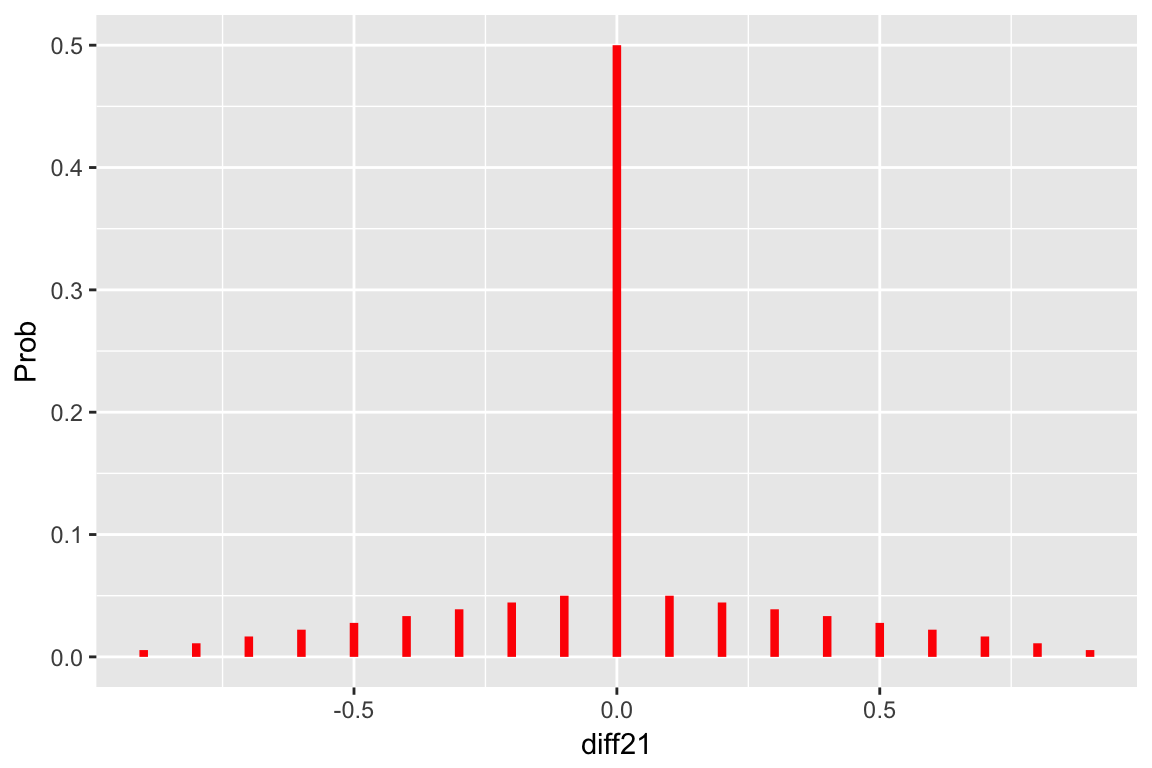
\includegraphics{bookdown-demo_files/figure-latex/unnamed-chunk-11-1.pdf}

A 90\% posterior interval estimate is found by selecting particular quantiles from the simulated values of \(p\).

\begin{Shaded}
\begin{Highlighting}[]
\KeywordTok{quantile}\NormalTok{(post}\OperatorTok{$}\NormalTok{p, }\KeywordTok{c}\NormalTok{(.}\DecValTok{05}\NormalTok{, }\FloatTok{.95}\NormalTok{))}
\end{Highlighting}
\end{Shaded}

\begin{verbatim}
##        5%       95% 
## 0.2378037 0.5192776
\end{verbatim}

\hypertarget{normal-modeling}{%
\chapter{Normal Modeling}\label{normal-modeling}}

\hypertarget{packages-for-example}{%
\section{Packages for example}\label{packages-for-example}}

\begin{Shaded}
\begin{Highlighting}[]
\KeywordTok{library}\NormalTok{(ProbBayes)}
\KeywordTok{library}\NormalTok{(brms)}
\end{Highlighting}
\end{Shaded}

\hypertarget{normal-sampling-model}{%
\section{Normal sampling model}\label{normal-sampling-model}}

Assume that \(y_1, ..., y_n\) are a sample from a normal distribution with mean \(\mu\) and standard deviation \(\sigma\).

For a prior, we assume that \(\mu\) and \(\sigma\) are independent where \(\mu\) is assigned a normal prior and \(\sigma\) is assigned a uniform prior on an interval.

\hypertarget{data-and-prior}{%
\section{Data and prior}\label{data-and-prior}}

We consider the variable \texttt{time} from the dataset \texttt{federer\_time\_to\_serve} that contains the time to serve for 20 serves of Roger Federer.

We place a weakly informative prior on the parameters. We assume the mean time-to-serve \(\mu\) is N(15, 5) and assume the standard deviation \(\sigma\) is uniform on the interval (0, 20).

\hypertarget{bayesian-fitting}{%
\section{Bayesian fitting}\label{bayesian-fitting}}

We use the \texttt{brm()} function with the family = gaussian option. Note how the prior is specified by the prior argument.

\begin{Shaded}
\begin{Highlighting}[]
\NormalTok{fit <-}\StringTok{ }\KeywordTok{brm}\NormalTok{(}\DataTypeTok{data =}\NormalTok{ federer_time_to_serve, }
            \DataTypeTok{family =}\NormalTok{ gaussian,}
\NormalTok{            time }\OperatorTok{~}\StringTok{ }\DecValTok{1}\NormalTok{,}
    \DataTypeTok{prior =} \KeywordTok{c}\NormalTok{(}\KeywordTok{prior}\NormalTok{(}\KeywordTok{normal}\NormalTok{(}\DecValTok{15}\NormalTok{, }\DecValTok{5}\NormalTok{), }\DataTypeTok{class =}\NormalTok{ Intercept),}
              \KeywordTok{prior}\NormalTok{(}\KeywordTok{uniform}\NormalTok{(}\DecValTok{0}\NormalTok{, }\DecValTok{20}\NormalTok{), }\DataTypeTok{class =}\NormalTok{ sigma)),}
    \DataTypeTok{iter =} \DecValTok{1000}\NormalTok{, }\DataTypeTok{refresh =} \DecValTok{0}\NormalTok{, }\DataTypeTok{chains =} \DecValTok{4}\NormalTok{)}
\end{Highlighting}
\end{Shaded}

\begin{verbatim}
## Warning: It appears as if you have specified an upper bounded prior on a parameter that has no natural upper bound.
## If this is really what you want, please specify argument 'ub' of 'set_prior' appropriately.
## Warning occurred for prior 
## sigma ~ uniform(0, 20)
\end{verbatim}

\begin{verbatim}
## Compiling Stan program...
\end{verbatim}

\begin{verbatim}
## Start sampling
\end{verbatim}

One obtains density plots and trace plots for \(\mu\) and \(\sigma\) by the \texttt{plot()} function.

\begin{Shaded}
\begin{Highlighting}[]
\KeywordTok{plot}\NormalTok{(fit)}
\end{Highlighting}
\end{Shaded}

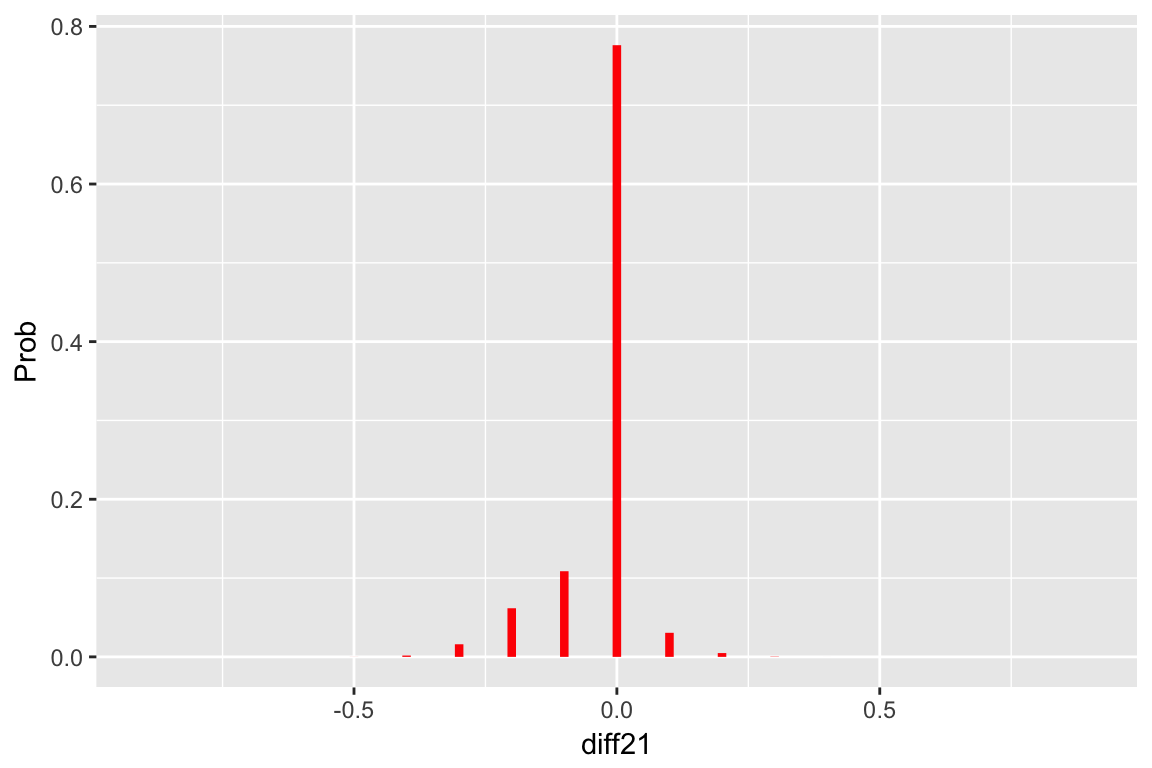
\includegraphics{bookdown-demo_files/figure-latex/unnamed-chunk-15-1.pdf}

One obtains posterior summaries for each parameter by the \texttt{summary()} function.

\begin{Shaded}
\begin{Highlighting}[]
\KeywordTok{summary}\NormalTok{(fit)}
\end{Highlighting}
\end{Shaded}

\begin{verbatim}
##  Family: gaussian 
##   Links: mu = identity; sigma = identity 
## Formula: time ~ 1 
##    Data: federer_time_to_serve (Number of observations: 20) 
## Samples: 4 chains, each with iter = 1000; warmup = 500; thin = 1;
##          total post-warmup samples = 2000
## 
## Population-Level Effects: 
##           Estimate Est.Error l-95% CI u-95% CI Rhat Bulk_ESS Tail_ESS
## Intercept    17.14      0.80    15.58    18.70 1.00     1394     1053
## 
## Family Specific Parameters: 
##       Estimate Est.Error l-95% CI u-95% CI Rhat Bulk_ESS Tail_ESS
## sigma     3.68      0.66     2.64     5.21 1.00     1137      878
## 
## Samples were drawn using sampling(NUTS). For each parameter, Bulk_ESS
## and Tail_ESS are effective sample size measures, and Rhat is the potential
## scale reduction factor on split chains (at convergence, Rhat = 1).
\end{verbatim}

One can obtain a matrix of simulated draws by the \texttt{posterior\_samples()} function.

\begin{Shaded}
\begin{Highlighting}[]
\NormalTok{post <-}\StringTok{ }\KeywordTok{posterior_samples}\NormalTok{(fit)}
\KeywordTok{head}\NormalTok{(post)}
\end{Highlighting}
\end{Shaded}

\begin{verbatim}
##   b_Intercept    sigma      lp__
## 1    17.69829 3.989865 -57.47744
## 2    17.47939 3.252316 -57.01475
## 3    15.76746 4.781054 -59.40308
## 4    17.62919 4.469536 -58.14521
## 5    16.42508 2.837153 -58.30991
## 6    18.14501 3.504918 -57.70406
\end{verbatim}

\hypertarget{poisson-modeling}{%
\chapter{Poisson Modeling}\label{poisson-modeling}}

\hypertarget{packages-for-example}{%
\section{Packages for example}\label{packages-for-example}}

\begin{Shaded}
\begin{Highlighting}[]
\KeywordTok{library}\NormalTok{(ProbBayes)}
\KeywordTok{library}\NormalTok{(brms)}
\end{Highlighting}
\end{Shaded}

\hypertarget{poisson-log-linear-model}{%
\section{Poisson log-linear model}\label{poisson-log-linear-model}}

Here we observe counts \(y_1, ..., y_n\) distributed according to a Poisson distribution with mean \(\lambda\).

Write a model in terms of the logarithm of the mean:

\[
\theta = \log \lambda
\]

Complete the model by assigning a \(N(\mu, \sigma)\) prior to the log mean parameter \(\theta\).

\hypertarget{learning-about-website-counts}{%
\section{Learning about website counts}\label{learning-about-website-counts}}

In the \texttt{ProbBayes} package, the variable \texttt{Count} in the dataset \texttt{web\_visits} contains counts of daily visits to a blog website. We are interested in learning about the mean count of visits \(\lambda\).

We place a N(0, 10) prior on \(\theta = \log \lambda\) reflecting weak prior information about the location of this paramter.

\hypertarget{bayesian-fitting}{%
\section{Bayesian Fitting}\label{bayesian-fitting}}

In this run of the \texttt{brm()} function, we assume Poisson sampling and a normal prior with mean 0 and standard deviation 10 placed on the log mean \(\theta = \log \lambda\).

\begin{Shaded}
\begin{Highlighting}[]
\NormalTok{fit <-}\StringTok{ }\KeywordTok{brm}\NormalTok{(Count }\OperatorTok{~}\StringTok{ }\DecValTok{0} \OperatorTok{+}\StringTok{ }\NormalTok{Intercept, }
            \DataTypeTok{data =}\NormalTok{ web_visits,}
            \DataTypeTok{family =}\NormalTok{ poisson,}
             \DataTypeTok{refresh =} \DecValTok{0}\NormalTok{,}
           \DataTypeTok{prior =} \KeywordTok{prior}\NormalTok{(}\KeywordTok{normal}\NormalTok{(}\DecValTok{0}\NormalTok{, }\DecValTok{10}\NormalTok{), }
                         \DataTypeTok{class =}\NormalTok{ b,}
                         \DataTypeTok{coef =} \StringTok{"Intercept"}\NormalTok{))}
\end{Highlighting}
\end{Shaded}

\begin{verbatim}
## Compiling Stan program...
\end{verbatim}

\begin{verbatim}
## Start sampling
\end{verbatim}

We confirm the prior with the \texttt{prior\_summary()} function.

\begin{Shaded}
\begin{Highlighting}[]
\KeywordTok{prior_summary}\NormalTok{(fit)}
\end{Highlighting}
\end{Shaded}

\begin{verbatim}
##           prior class      coef group resp dpar nlpar bound
## 1                   b                                      
## 2 normal(0, 10)     b Intercept
\end{verbatim}

The \texttt{summary()} function provides summaries of the posterior of \(\theta\).

\begin{Shaded}
\begin{Highlighting}[]
\KeywordTok{summary}\NormalTok{(fit)}
\end{Highlighting}
\end{Shaded}

\begin{verbatim}
##  Family: poisson 
##   Links: mu = log 
## Formula: Count ~ 0 + Intercept 
##    Data: web_visits (Number of observations: 28) 
## Samples: 4 chains, each with iter = 2000; warmup = 1000; thin = 1;
##          total post-warmup samples = 4000
## 
## Population-Level Effects: 
##           Estimate Est.Error l-95% CI u-95% CI Rhat Bulk_ESS Tail_ESS
## Intercept     4.59      0.02     4.55     4.62 1.00     1574     2209
## 
## Samples were drawn using sampling(NUTS). For each parameter, Bulk_ESS
## and Tail_ESS are effective sample size measures, and Rhat is the potential
## scale reduction factor on split chains (at convergence, Rhat = 1).
\end{verbatim}

The \texttt{posterior\_samples()} function outputs the posterior simulations of \(\theta\).

\begin{Shaded}
\begin{Highlighting}[]
\NormalTok{post <-}\StringTok{ }\KeywordTok{posterior_samples}\NormalTok{(fit)}
\KeywordTok{head}\NormalTok{(post)}
\end{Highlighting}
\end{Shaded}

\begin{verbatim}
##   b_Intercept      lp__
## 1    4.556476 -136.7185
## 2    4.562960 -136.2752
## 3    4.560979 -136.3987
## 4    4.598670 -135.8759
## 5    4.594855 -135.7515
## 6    4.590376 -135.6570
\end{verbatim}

\hypertarget{posterior-predictive-model-checks}{%
\section{Posterior predictive model checks}\label{posterior-predictive-model-checks}}

Actual this is a poor model for these data. One can see that by several posterior predictive checks.

The \texttt{pp\_check()} shows density plots of 10 replicated datasets from the posterior predictive distribution. Note that these replicated datasets look different (smaller variation) than the observed data.

\begin{Shaded}
\begin{Highlighting}[]
\KeywordTok{pp_check}\NormalTok{(fit)}
\end{Highlighting}
\end{Shaded}

\begin{verbatim}
## Using 10 posterior samples for ppc type 'dens_overlay' by default.
\end{verbatim}

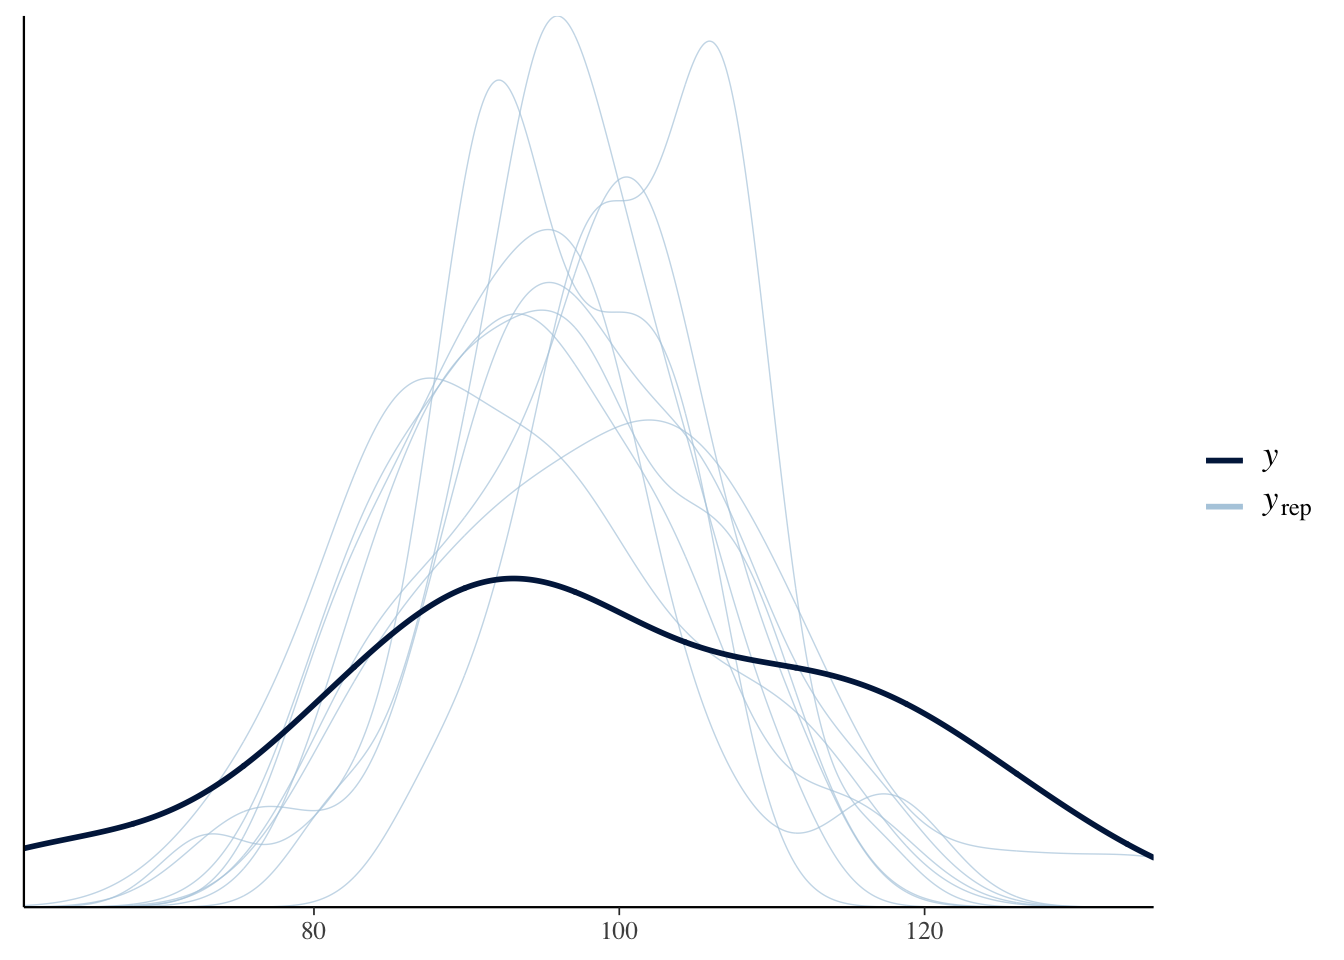
\includegraphics{bookdown-demo_files/figure-latex/unnamed-chunk-23-1.pdf}

The \texttt{pp\_check()} function will implement a posterior predictive check using various checking functions. Here we are using \((\bar y, s)\) as a bivariate checking function. The scatterplot represents values of \((\bar y, s)\) from the simulated predictive distributions and the observed values of \((\bar y, s)\) is displayed. The takeaway is that the observed data has more variation than predicted from the Poisson model.

\begin{Shaded}
\begin{Highlighting}[]
\KeywordTok{pp_check}\NormalTok{(fit, }\DataTypeTok{type =} \StringTok{"stat_2d"}\NormalTok{)}
\end{Highlighting}
\end{Shaded}

\begin{verbatim}
## Using all posterior samples for ppc type 'stat_2d' by default.
\end{verbatim}

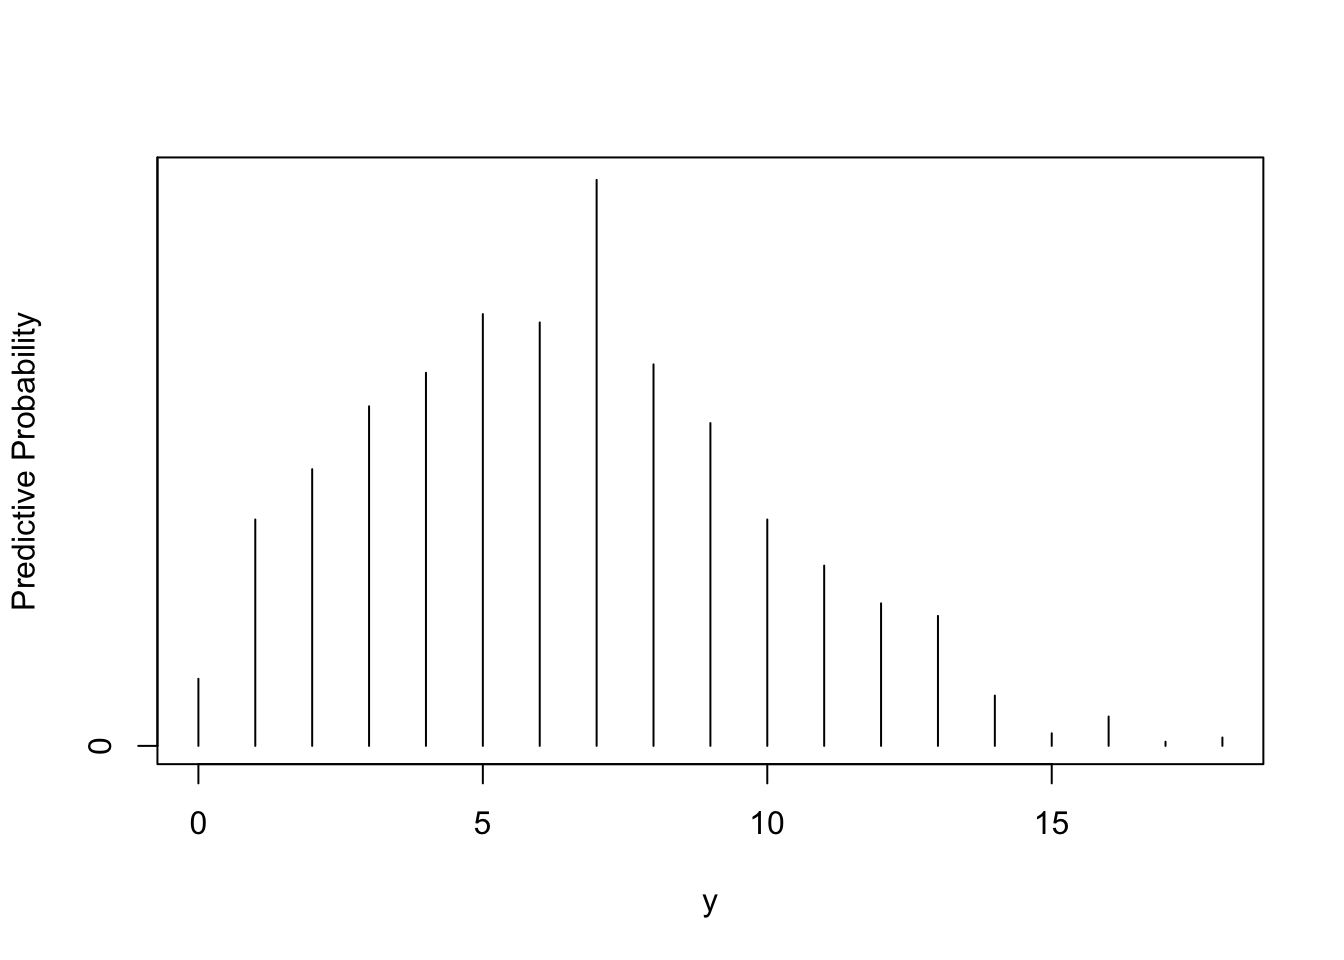
\includegraphics{bookdown-demo_files/figure-latex/unnamed-chunk-24-1.pdf}

\hypertarget{comparing-proportions}{%
\chapter{Comparing Proportions}\label{comparing-proportions}}

\hypertarget{packages-for-example}{%
\section{Packages for example}\label{packages-for-example}}

\begin{Shaded}
\begin{Highlighting}[]
\KeywordTok{library}\NormalTok{(ProbBayes)}
\KeywordTok{library}\NormalTok{(brms)}
\KeywordTok{library}\NormalTok{(dplyr)}
\KeywordTok{library}\NormalTok{(ggplot2)}
\end{Highlighting}
\end{Shaded}

\hypertarget{facebook-use-example}{%
\section{Facebook use example}\label{facebook-use-example}}

In Chapter 9, we consider the following comparison of proportions example. A sample of students were asked their gender and the average number of times they visited Facebook in a day.

Of \(n_M\) males sampled, \(y_M\) had a high number of Facebook visits, and of \(n_F\) females sampled, \(y_F\) had a high number of visits.

Suppose the data is organized as a data frame as follows:

\begin{longtable}[]{@{}lll@{}}
\toprule
Gender & Sample\_size & Visits\tabularnewline
\midrule
\endhead
male & \(n_M\) & \(y_M\)\tabularnewline
female & \(n_F\) & \(y_F\)\tabularnewline
\bottomrule
\end{longtable}

\hypertarget{sampling-model}{%
\section{Sampling model}\label{sampling-model}}

Suppose we have two independent samples where \(y_M\) is binomial(\(n_M, p_M\)) and \(y_F\) is binomial(\(n_F, p_F\)).

Write the proportions using a logistic model:

\[
\log\left(\frac{p}{1-p}\right) = \beta_0 + \beta_1 I(Gender = Male)
\]

Note for females, the logit of \(p_F\) is given by
\[
\log\left(\frac{p}{1-p}\right) = \beta_0
\]
and for males the logit for \(p_M\) is given by
\[
\log\left(\frac{p}{1-p}\right) = \beta_0 + \beta_1
\]

\hypertarget{the-data}{%
\section{The data}\label{the-data}}

Here's the observed data:

\begin{Shaded}
\begin{Highlighting}[]
\NormalTok{fb_data <-}\StringTok{ }\KeywordTok{data.frame}\NormalTok{(}\DataTypeTok{Gender =} \KeywordTok{c}\NormalTok{(}\StringTok{"male"}\NormalTok{, }\StringTok{"female"}\NormalTok{),}
                      \DataTypeTok{Sample_Size =} \KeywordTok{c}\NormalTok{(}\DecValTok{93}\NormalTok{, }\DecValTok{151}\NormalTok{),}
                      \DataTypeTok{Visits =} \KeywordTok{c}\NormalTok{(}\DecValTok{39}\NormalTok{, }\DecValTok{75}\NormalTok{))}
\end{Highlighting}
\end{Shaded}

\hypertarget{priors}{%
\section{Priors}\label{priors}}

In this model, \(\beta_0\) is the logit of the proportion of women who are high Facebook users and \(\beta_1\) represents the difference in the logits of the proportions for men and women.

Assume that you don't know much about the location of \(\beta_0\), but you believe men and women are similar in their use of Facebook. So you assign a N(0, 31.6) prior to \(\beta_0\) with a high standard deviation, reflecting little knowledge. To reflect the belief that \(\beta_1\) is close to 0, you use a N(0, 0.71) prior.

The \texttt{get\_prior()} function lists all parameters to define priors on for this particular model, assigning the result to \texttt{prior}. Then the two components of \texttt{prior} are assigned that reflect the statements above.

\begin{Shaded}
\begin{Highlighting}[]
\NormalTok{(my_prior <-}\StringTok{ }\KeywordTok{get_prior}\NormalTok{(}\DataTypeTok{family =}\NormalTok{ binomial,}
\NormalTok{           Visits }\OperatorTok{|}\StringTok{ }\KeywordTok{trials}\NormalTok{(Sample_Size) }\OperatorTok{~}\StringTok{ }\NormalTok{Gender,}
           \DataTypeTok{data =}\NormalTok{ fb_data))}
\end{Highlighting}
\end{Shaded}

\begin{verbatim}
##                  prior     class       coef group resp dpar nlpar bound
## 1                              b                                       
## 2                              b Gendermale                            
## 3 student_t(3, 0, 2.5) Intercept
\end{verbatim}

\begin{Shaded}
\begin{Highlighting}[]
\NormalTok{my_prior}\OperatorTok{$}\NormalTok{prior[}\DecValTok{3}\NormalTok{] <-}\StringTok{ "normal(0, 31.6)"}
\NormalTok{my_prior}\OperatorTok{$}\NormalTok{prior[}\DecValTok{2}\NormalTok{] <-}\StringTok{ "normal(0, 0.71)"}
\end{Highlighting}
\end{Shaded}

\hypertarget{posterior-sampling}{%
\section{Posterior sampling}\label{posterior-sampling}}

Here is the run of \texttt{brm()} where I use the prior specification in \texttt{my\_prior}.

\begin{Shaded}
\begin{Highlighting}[]
\NormalTok{fit <-}\StringTok{ }\KeywordTok{brm}\NormalTok{(}\DataTypeTok{family =}\NormalTok{ binomial,}
\NormalTok{           Visits }\OperatorTok{|}\StringTok{ }\KeywordTok{trials}\NormalTok{(Sample_Size) }\OperatorTok{~}\StringTok{ }\NormalTok{Gender,}
           \DataTypeTok{data =}\NormalTok{ fb_data,}
           \DataTypeTok{prior =}\NormalTok{ my_prior,}
           \DataTypeTok{iter =} \DecValTok{1000}\NormalTok{,}
           \DataTypeTok{refresh =} \DecValTok{0}\NormalTok{)}
\end{Highlighting}
\end{Shaded}

\begin{verbatim}
## Compiling Stan program...
\end{verbatim}

\begin{verbatim}
## Start sampling
\end{verbatim}

One obtains the matrix of simulated values of the parameters by the \texttt{posterior\_samples()} function.

\begin{Shaded}
\begin{Highlighting}[]
\NormalTok{post <-}\StringTok{ }\KeywordTok{posterior_samples}\NormalTok{(fit)}
\KeywordTok{head}\NormalTok{(post)}
\end{Highlighting}
\end{Shaded}

\begin{verbatim}
##    b_Intercept b_Gendermale      lp__
## 1  0.149825204   -0.3929578 -10.89798
## 2 -0.077477237   -0.1550768 -10.36612
## 3  0.014914205   -0.2591160 -10.32287
## 4 -0.244104208   -0.2079800 -11.39275
## 5 -0.006092644   -0.2035093 -10.36111
## 6  0.012292753   -0.4538551 -10.53464
\end{verbatim}

The \texttt{plot()} function provides trace plots and density plots of each parameter.

\begin{Shaded}
\begin{Highlighting}[]
\KeywordTok{plot}\NormalTok{(fit)}
\end{Highlighting}
\end{Shaded}

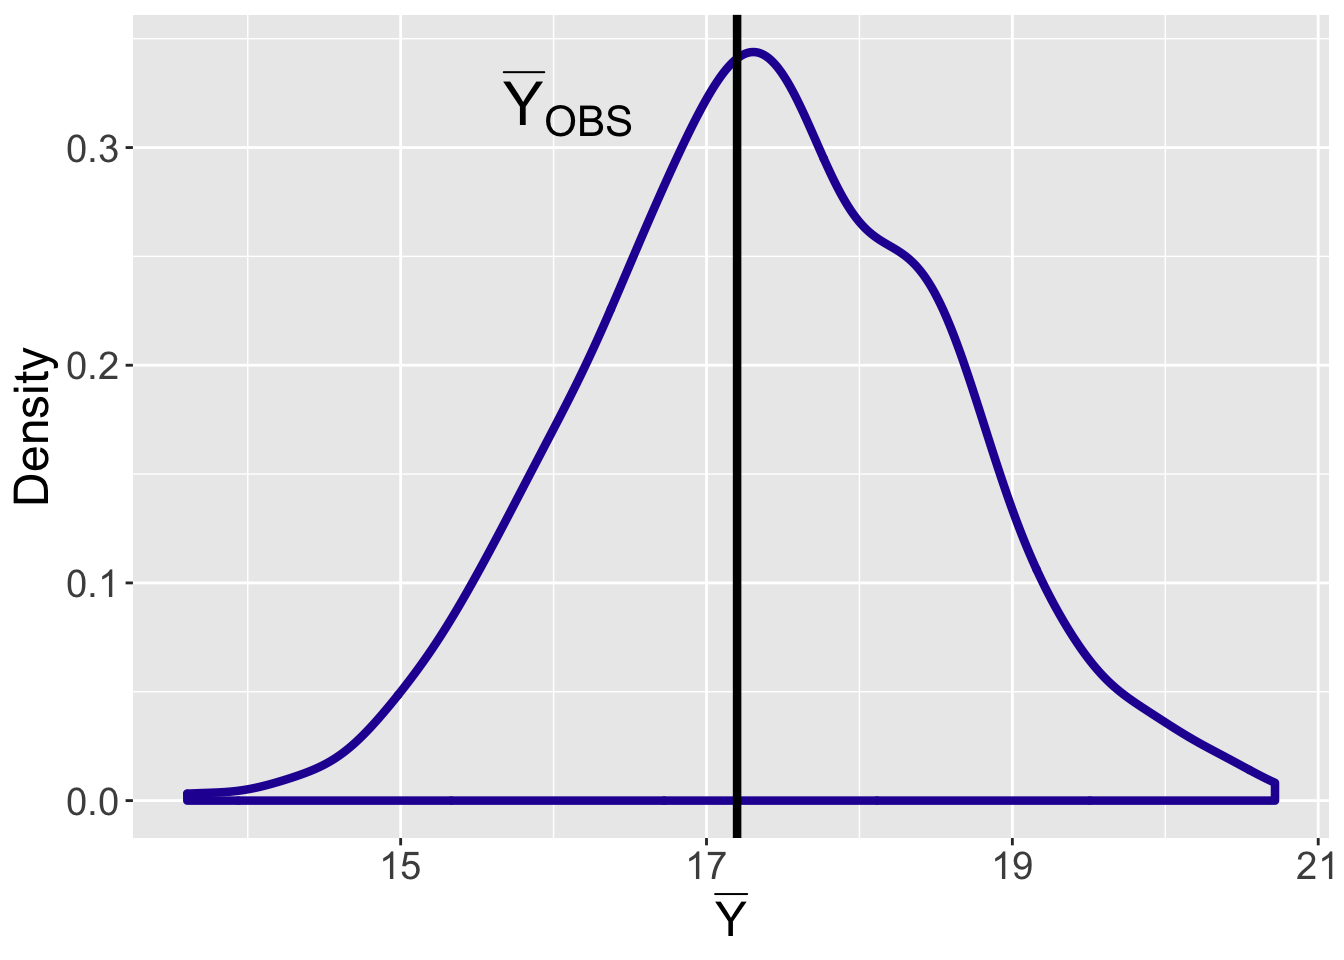
\includegraphics{bookdown-demo_files/figure-latex/unnamed-chunk-31-1.pdf}

Posterior summaries are provided by the \texttt{print()} function.

\begin{Shaded}
\begin{Highlighting}[]
\KeywordTok{print}\NormalTok{(fit)}
\end{Highlighting}
\end{Shaded}

\begin{verbatim}
##  Family: binomial 
##   Links: mu = logit 
## Formula: Visits | trials(Sample_Size) ~ Gender 
##    Data: fb_data (Number of observations: 2) 
## Samples: 4 chains, each with iter = 1000; warmup = 500; thin = 1;
##          total post-warmup samples = 2000
## 
## Population-Level Effects: 
##            Estimate Est.Error l-95% CI u-95% CI Rhat Bulk_ESS Tail_ESS
## Intercept     -0.03      0.16    -0.34     0.28 1.00     2198     1576
## Gendermale    -0.28      0.25    -0.78     0.23 1.01     1525     1121
## 
## Samples were drawn using sampling(NUTS). For each parameter, Bulk_ESS
## and Tail_ESS are effective sample size measures, and Rhat is the potential
## scale reduction factor on split chains (at convergence, Rhat = 1).
\end{verbatim}

\hypertarget{comparing-rates}{%
\chapter{Comparing Rates}\label{comparing-rates}}

\hypertarget{packages-for-example}{%
\section{Packages for example}\label{packages-for-example}}

\begin{Shaded}
\begin{Highlighting}[]
\KeywordTok{library}\NormalTok{(ProbBayes)}
\KeywordTok{library}\NormalTok{(brms)}
\KeywordTok{library}\NormalTok{(dplyr)}
\end{Highlighting}
\end{Shaded}

\hypertarget{comparing-two-poisson-rates}{%
\section{Comparing two Poisson Rates}\label{comparing-two-poisson-rates}}

Suppose we observe two independent samples: \(x_1, ..., x_m\) are a random sample from a Poisson distribution with mean \(\lambda_x\), and \(w_1, ..., w_n\) are a random sample from a Poisson distribution with mean \(\lambda_y\). We are interested in learning about the ratio of Poisson means
\[
\theta = \frac{\lambda_x}{\lambda_y}
\]

\hypertarget{write-as-a-log-linear-model}{%
\section{Write as a log-linear model}\label{write-as-a-log-linear-model}}

Suppose we collect the observations
\[
y = c(x_1, ..., x_m, w_1, ..., w_n)
\]
and let \texttt{group2} be an indicator variable for the second group.
\[
group2 = c(0, 0, ..., 0, 1, 1, ..., 1)
\]
Then we can represent the model as
\[
y_1, ..., y_{m+n}
\]
independent from Poisson distributions with means \(\lambda_1, ..., \lambda_{m_n}\) where the means follow the log-linear model
\[
\log \lambda_j = \beta_0 + \beta_1 group2
\]

In this model, \(\beta_0 = \log \lambda_x\), and \(\beta_0 + \beta_1 = \log \lambda_y\). So \(\beta_1 = \log(\lambda_y) - \log(\lambda_x)\) represents the increase in the means on the log scale.

\hypertarget{the-data}{%
\section{The data}\label{the-data}}

We collect web count visits for a number of days stored in the data frame \texttt{web\_visits} in the \texttt{ProbBayes} package. The key variables are \texttt{Day}, the day of the week, and \texttt{Count}, the website visit count. We define a new variable \texttt{Type} that is either ``weekend'' or ``weekday''.

We are interested in comparing the mean visit counts for weekdays and weekend days.

\begin{Shaded}
\begin{Highlighting}[]
\NormalTok{web_visits }\OperatorTok\StringTok{ }
\StringTok{  }\KeywordTok{mutate}\NormalTok{(}\DataTypeTok{Type =} \KeywordTok{ifelse}\NormalTok{(Day }\OperatorTok\StringTok{ }
\StringTok{      }\KeywordTok{c}\NormalTok{(}\StringTok{"Fri"}\NormalTok{, }\StringTok{"Sat"}\NormalTok{, }\StringTok{"Sun"}\NormalTok{), }\StringTok{"weekend"}\NormalTok{, }\StringTok{"weekday"}\NormalTok{)) ->}\StringTok{ }\NormalTok{web_visits}
\end{Highlighting}
\end{Shaded}

\hypertarget{priors}{%
\section{Priors}\label{priors}}

Here we are assume weakly informative priors on the regression parameters \(\beta_0\) and \(\beta_1\).

\hypertarget{bayesian-fitting}{%
\section{Bayesian fitting}\label{bayesian-fitting}}

\begin{Shaded}
\begin{Highlighting}[]
\NormalTok{fit <-}\StringTok{ }\KeywordTok{brm}\NormalTok{(Count }\OperatorTok{~}\StringTok{ }\NormalTok{Type,}
           \DataTypeTok{family =}\NormalTok{ poisson,}
           \DataTypeTok{data =}\NormalTok{ web_visits,}
           \DataTypeTok{refresh =} \DecValTok{0}\NormalTok{)}
\end{Highlighting}
\end{Shaded}

\begin{verbatim}
## Compiling Stan program...
\end{verbatim}

\begin{verbatim}
## Start sampling
\end{verbatim}

\begin{Shaded}
\begin{Highlighting}[]
\KeywordTok{plot}\NormalTok{(fit)}
\end{Highlighting}
\end{Shaded}

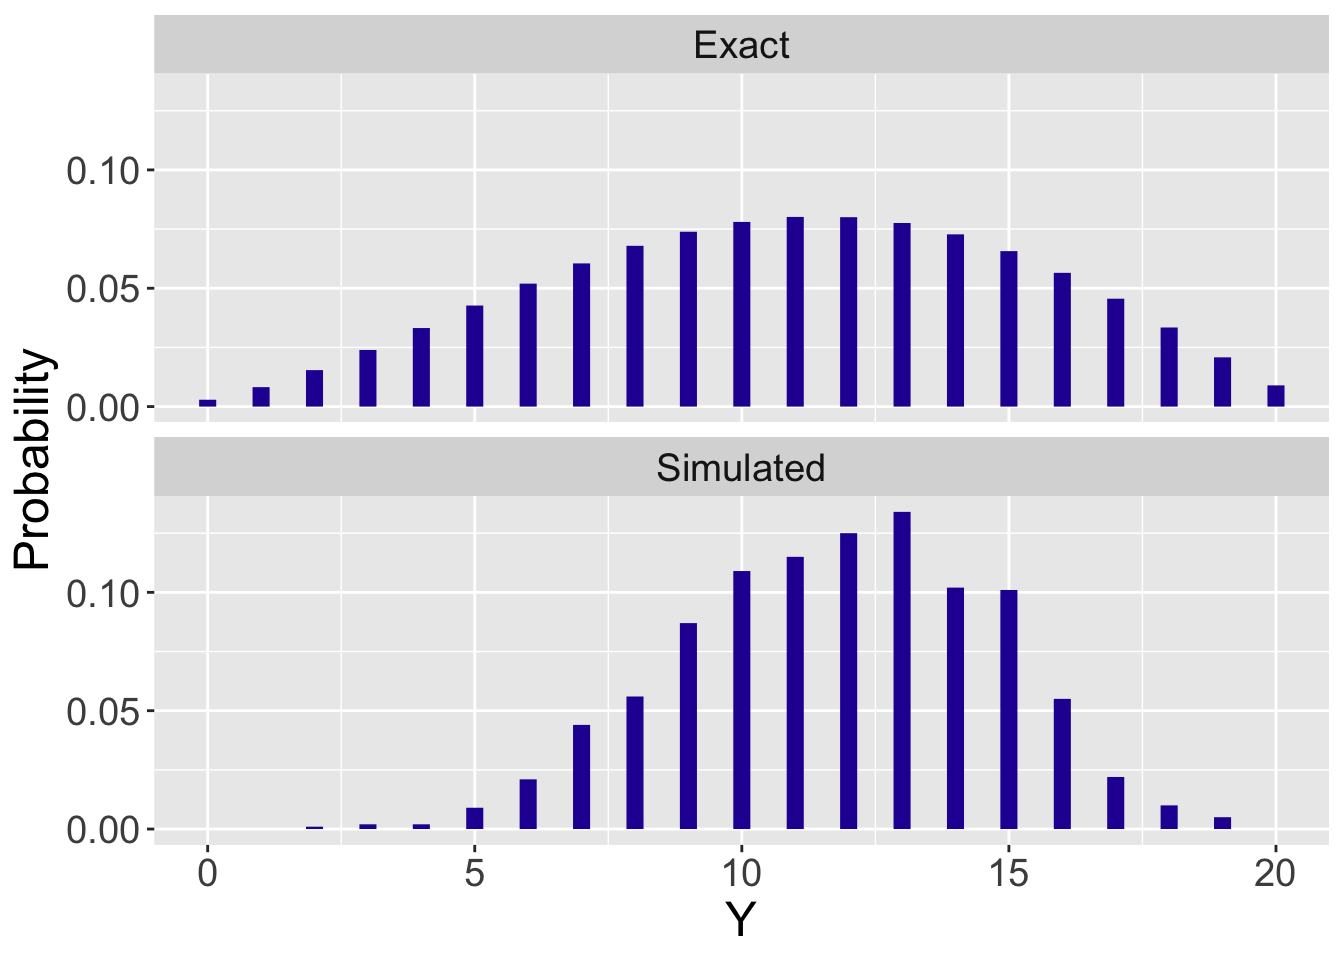
\includegraphics{bookdown-demo_files/figure-latex/unnamed-chunk-36-1.pdf}

\begin{Shaded}
\begin{Highlighting}[]
\KeywordTok{summary}\NormalTok{(fit)}
\end{Highlighting}
\end{Shaded}

\begin{verbatim}
##  Family: poisson 
##   Links: mu = log 
## Formula: Count ~ Type 
##    Data: web_visits (Number of observations: 28) 
## Samples: 4 chains, each with iter = 2000; warmup = 1000; thin = 1;
##          total post-warmup samples = 4000
## 
## Population-Level Effects: 
##             Estimate Est.Error l-95% CI u-95% CI Rhat Bulk_ESS Tail_ESS
## Intercept       4.69      0.02     4.64     4.74 1.00     3888     2663
## Typeweekend    -0.27      0.04    -0.35    -0.19 1.00     3292     2805
## 
## Samples were drawn using sampling(NUTS). For each parameter, Bulk_ESS
## and Tail_ESS are effective sample size measures, and Rhat is the potential
## scale reduction factor on split chains (at convergence, Rhat = 1).
\end{verbatim}

\begin{Shaded}
\begin{Highlighting}[]
\NormalTok{sim_draws <-}\StringTok{ }\KeywordTok{posterior_samples}\NormalTok{(fit)}
\KeywordTok{head}\NormalTok{(sim_draws)}
\end{Highlighting}
\end{Shaded}

\begin{verbatim}
##   b_Intercept b_Typeweekend      lp__
## 1    4.683972    -0.3003928 -111.6071
## 2    4.690432    -0.2403990 -111.1721
## 3    4.665176    -0.2213930 -111.6114
## 4    4.683088    -0.2696015 -110.9016
## 5    4.678049    -0.2929583 -111.6562
## 6    4.699903    -0.2566505 -111.0721
\end{verbatim}

\hypertarget{multilevel-modeling-of-proportions}{%
\chapter{Multilevel Modeling of Proportions}\label{multilevel-modeling-of-proportions}}

\hypertarget{packages-for-example}{%
\section{Packages for example}\label{packages-for-example}}

\begin{Shaded}
\begin{Highlighting}[]
\KeywordTok{library}\NormalTok{(ProbBayes)}
\KeywordTok{library}\NormalTok{(tidyverse)}
\KeywordTok{library}\NormalTok{(brms)}
\end{Highlighting}
\end{Shaded}

\hypertarget{hospital-study}{%
\section{Hospital Study}\label{hospital-study}}

Table 10.2 gives the number of cases and number of deaths from heart attacks for 13 hospitals in New York City. This data is contained in the data frame \texttt{DeathHeartAttackManhattan} in the \texttt{ProbBayes} package.

\hypertarget{a-multilevel-model}{%
\section{A Multilevel Model}\label{a-multilevel-model}}

We consider a different formulation of the hierarchical model described in Section 10.3.

\textbf{Sampling}

We first assume that \(y_j\), the number of deaths for the \(j\)th hospital, is binomial with sample size \(n_j\) and probability \(p_j\). Let \(\theta_j = \log (p_j / (1 - p_j))\) denote the logit for the \(j\)th hospital.

Write \(\theta_j = \beta + \gamma_j\).

\textbf{Prior}

\begin{enumerate}
\def\labelenumi{\arabic{enumi}.}
\item
  We assume the intercept \(\beta\) has a student t distribution with mean 0, scale parameter 2.5 and 3 degrees of freedom.
\item
  We assume \(\gamma_1, ..., \gamma_N\) have a normal distribution with mean 0 and standard deviation \(\sigma\).
\item
  The standard deviation \(\sigma\) is assumed to have a t density with mean 0 and standard deviation 3.5.
\end{enumerate}

\hypertarget{fitting-the-bayesian-model}{%
\section{Fitting the Bayesian model}\label{fitting-the-bayesian-model}}

We fit the multilevel model using the `\texttt{brm()} function. Note the use of the ``family = binomial'' argument to indicate the sampling distribution. The ``(1 \textbar{} Hospital)'' component indicates that the \(\gamma_j\) have a random distribution.

\begin{Shaded}
\begin{Highlighting}[]
\NormalTok{fit <-}\StringTok{ }\KeywordTok{brm}\NormalTok{(}\DataTypeTok{data =}\NormalTok{ DeathHeartAttackManhattan, }
           \DataTypeTok{family =}\NormalTok{ binomial,}
\NormalTok{           Deaths }\OperatorTok{|}\StringTok{ }\KeywordTok{trials}\NormalTok{(Cases) }\OperatorTok{~}\StringTok{ }\DecValTok{1} \OperatorTok{+}\StringTok{ }\NormalTok{(}\DecValTok{1} \OperatorTok{|}\StringTok{ }\NormalTok{Hospital),}
           \DataTypeTok{refresh =} \DecValTok{0}\NormalTok{)}
\end{Highlighting}
\end{Shaded}

\begin{verbatim}
## Compiling Stan program...
\end{verbatim}

\begin{verbatim}
## Start sampling
\end{verbatim}

We didn't specify priors, but there are default priors behind the scenes. The \texttt{prior\_summary()} function displays the priors.

\begin{Shaded}
\begin{Highlighting}[]
\KeywordTok{prior_summary}\NormalTok{(fit)}
\end{Highlighting}
\end{Shaded}

\begin{verbatim}
##                  prior     class      coef    group resp dpar nlpar bound
## 1 student_t(3, 0, 2.5) Intercept                                         
## 2 student_t(3, 0, 2.5)        sd                                         
## 3                             sd           Hospital                      
## 4                             sd Intercept Hospital
\end{verbatim}

\hypertarget{posterior-summaries-of-beta-and-sigma}{%
\section{\texorpdfstring{Posterior summaries of \(\beta\) and \(\sigma\)}{Posterior summaries of \textbackslash beta and \textbackslash sigma}}\label{posterior-summaries-of-beta-and-sigma}}

The \texttt{summary()} function shows posterior summaries of \(\beta\) (the intercept) and the standard deviation \(\sigma\).

\begin{Shaded}
\begin{Highlighting}[]
\KeywordTok{summary}\NormalTok{(fit)}
\end{Highlighting}
\end{Shaded}

\begin{verbatim}
##  Family: binomial 
##   Links: mu = logit 
## Formula: Deaths | trials(Cases) ~ 1 + (1 | Hospital) 
##    Data: DeathHeartAttackManhattan (Number of observations: 13) 
## Samples: 4 chains, each with iter = 2000; warmup = 1000; thin = 1;
##          total post-warmup samples = 4000
## 
## Group-Level Effects: 
## ~Hospital (Number of levels: 13) 
##               Estimate Est.Error l-95% CI u-95% CI Rhat Bulk_ESS Tail_ESS
## sd(Intercept)     0.19      0.15     0.01     0.56 1.00      913     1675
## 
## Population-Level Effects: 
##           Estimate Est.Error l-95% CI u-95% CI Rhat Bulk_ESS Tail_ESS
## Intercept    -2.60      0.11    -2.82    -2.37 1.00     2555     1376
## 
## Samples were drawn using sampling(NUTS). For each parameter, Bulk_ESS
## and Tail_ESS are effective sample size measures, and Rhat is the potential
## scale reduction factor on split chains (at convergence, Rhat = 1).
\end{verbatim}

\hypertarget{posterior-summaries-of-hospital-effects}{%
\section{Posterior summaries of hospital effects}\label{posterior-summaries-of-hospital-effects}}

The \texttt{posterior\_samples()} function produces a large matrix of simulated draws where the column corresponds to the parameter and the row corresponds to the iteration number.

By use of the \texttt{pivot\_longer()} function, I reformat the simulation matrix where there is a new variable \texttt{Hospital} indicating the name of the hospital and \texttt{Effect} is the simulated value of \(\gamma_j\). Also I create a new variable that is the number of the hospital from 1 to 13.

\begin{Shaded}
\begin{Highlighting}[]
\KeywordTok{posterior_samples}\NormalTok{(fit) }\OperatorTok\StringTok{ }
\StringTok{  }\KeywordTok{pivot_longer}\NormalTok{(}\KeywordTok{starts_with}\NormalTok{(}\StringTok{"r_Hospital"}\NormalTok{),}
               \DataTypeTok{names_to =} \StringTok{"Hospital"}\NormalTok{,}
               \DataTypeTok{values_to =} \StringTok{"Effect"}\NormalTok{) ->}\StringTok{ }\NormalTok{post}
\NormalTok{post}\OperatorTok{$}\NormalTok{Hospital_No <-}\StringTok{ }\KeywordTok{as.character}\NormalTok{(}\KeywordTok{as.numeric}\NormalTok{(}\KeywordTok{factor}\NormalTok{(post}\OperatorTok{$}\NormalTok{Hospital)))}
\end{Highlighting}
\end{Shaded}

Below is a graph of the posterior distribution of the parameters \{\(\beta + \gamma_j\)\} for all 13 hospitals.

These are graphed on the logit scale. By taking the inverse logit function, one could find the posterior distributions of the death rates \(p_1, ..., p_N\).

\begin{Shaded}
\begin{Highlighting}[]
\KeywordTok{ggplot}\NormalTok{(post, }\KeywordTok{aes}\NormalTok{(Hospital_No, Effect }\OperatorTok{+}\StringTok{ }\NormalTok{b_Intercept)) }\OperatorTok{+}
\StringTok{  }\KeywordTok{geom_boxplot}\NormalTok{() }\OperatorTok{+}
\StringTok{  }\KeywordTok{coord_flip}\NormalTok{()}
\end{Highlighting}
\end{Shaded}

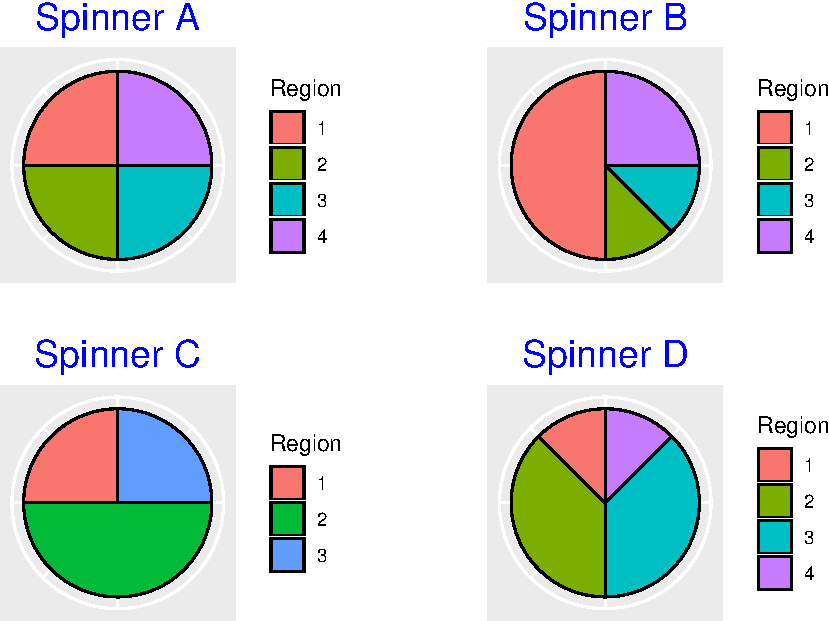
\includegraphics{bookdown-demo_files/figure-latex/unnamed-chunk-44-1.pdf}

\hypertarget{multilevel-modeling-of-means}{%
\chapter{Multilevel Modeling of Means}\label{multilevel-modeling-of-means}}

\hypertarget{packages-for-example}{%
\section{Packages for example}\label{packages-for-example}}

\begin{Shaded}
\begin{Highlighting}[]
\KeywordTok{library}\NormalTok{(ProbBayes)}
\KeywordTok{library}\NormalTok{(tidyverse)}
\KeywordTok{library}\NormalTok{(brms)}
\end{Highlighting}
\end{Shaded}

\hypertarget{movie-ratings-study}{%
\section{Movie Ratings Study}\label{movie-ratings-study}}

Table 10.1 gives summaries of the ratings for eight different animation movies. The table includes the number of ratings, the mean and the standard deviation of the ratings. The data is contained in the data frame \texttt{animation\_ratings} in the \texttt{ProbBayes} package.

\hypertarget{the-multilevel-model}{%
\section{The Multilevel Model}\label{the-multilevel-model}}

\textbf{Sampling}

Let \(y_{ij}\) denote the rating of the \(i\)th individual for the \(j\)th movie.

We assume that \(y_{ij} \sim N(\mu_j, \sigma)\).

\textbf{Prior}

The parameters \(\mu_1, ..., \mu_8\) represent the mean ratings for the eight movies. Write
\[
\mu_j = \beta + \gamma_j
\]

\begin{enumerate}
\def\labelenumi{\arabic{enumi}.}
\item
  The intercept parameter \(\beta\) has a student t distribution with mean 4, scale parameter 2.5, and 3 degrees of freedom.
\item
  We assume the effect parameters \(\gamma_1, ..., \gamma_8\) have a normal distribution with mean 0 and standard deviation \(\tau\).
\item
  There are two standard deviations, the sampling standard deviation \(\sigma\) and the between-means standard deviation \(\tau\). Each of these standard deviations are given weakly informative student t distributions with mean 0, scale 2.5 and 3 degrees of freedom.
\end{enumerate}

\hypertarget{bayesian-fitting}{%
\section{Bayesian Fitting}\label{bayesian-fitting}}

The model is fit by use of the \texttt{brm()} function. By default, this function assumes a Gaussian (normal) sampling distribution. The ``(1 \textbar{} movieID)'' argument indicates that the \(\mu_1, ..., \mu_8\) have a random distribution.

\begin{Shaded}
\begin{Highlighting}[]
\NormalTok{fit <-}\StringTok{ }\KeywordTok{brm}\NormalTok{(rating }\OperatorTok{~}\StringTok{ }\NormalTok{(}\DecValTok{1} \OperatorTok{|}\StringTok{ }\NormalTok{movieId),}
           \DataTypeTok{data =}\NormalTok{ animation_ratings,}
           \DataTypeTok{refresh =} \DecValTok{0}\NormalTok{)}
\end{Highlighting}
\end{Shaded}

\begin{verbatim}
## Compiling Stan program...
\end{verbatim}

\begin{verbatim}
## Start sampling
\end{verbatim}

\begin{verbatim}
## Warning: There were 6 divergent transitions after warmup. Increasing adapt_delta above 0.8 may help. See
## http://mc-stan.org/misc/warnings.html#divergent-transitions-after-warmup
\end{verbatim}

\begin{verbatim}
## Warning: Examine the pairs() plot to diagnose sampling problems
\end{verbatim}

One can check the default priors by use of the \texttt{prior\_summary()} function.

\begin{Shaded}
\begin{Highlighting}[]
\KeywordTok{prior_summary}\NormalTok{(fit)}
\end{Highlighting}
\end{Shaded}

\begin{verbatim}
##                  prior     class      coef   group resp dpar nlpar bound
## 1 student_t(3, 4, 2.5) Intercept                                        
## 2 student_t(3, 0, 2.5)        sd                                        
## 3                             sd           movieId                      
## 4                             sd Intercept movieId                      
## 5 student_t(3, 0, 2.5)     sigma
\end{verbatim}

The posterior matrix of simulated draws is available by use of the \texttt{posterior\_samples()} function. Below I construct density estimates of the two standard deviation parameters \(\sigma\) (blue) and \(\tau\) (red).

\begin{Shaded}
\begin{Highlighting}[]
\KeywordTok{ggplot}\NormalTok{(}\KeywordTok{posterior_samples}\NormalTok{(fit),}
       \KeywordTok{aes}\NormalTok{(sigma)) }\OperatorTok{+}
\StringTok{  }\KeywordTok{geom_density}\NormalTok{(}\DataTypeTok{color =} \StringTok{"blue"}\NormalTok{) }\OperatorTok{+}
\StringTok{  }\KeywordTok{geom_density}\NormalTok{(}\KeywordTok{aes}\NormalTok{(sd_movieId__Intercept),}
               \DataTypeTok{color =} \StringTok{"red"}\NormalTok{)}
\end{Highlighting}
\end{Shaded}

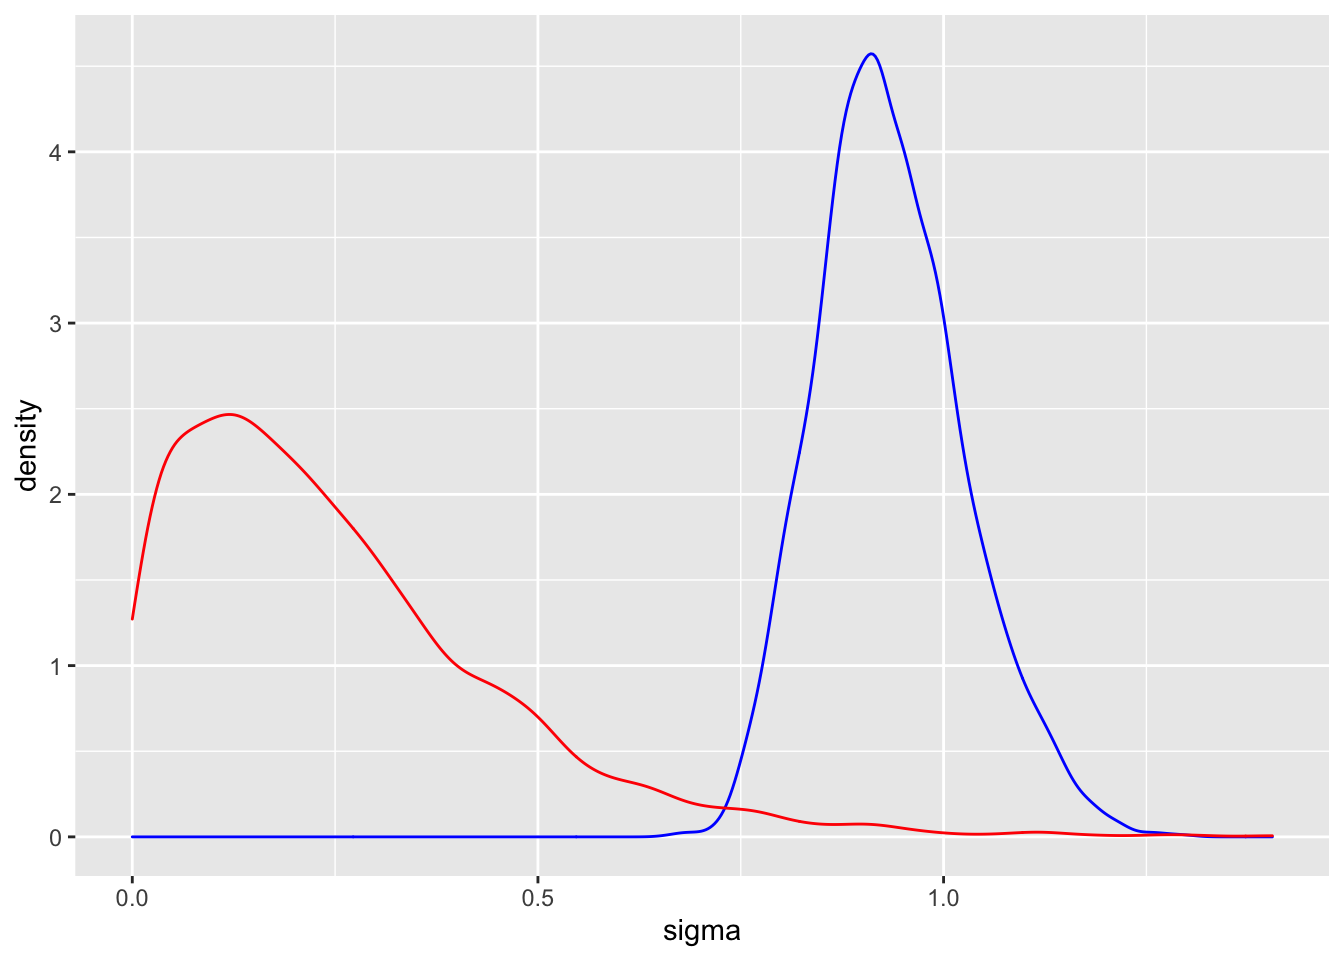
\includegraphics{bookdown-demo_files/figure-latex/unnamed-chunk-48-1.pdf}

To show the posterior distributions of the means, I reshape the matrix of simulated draws by use of the \texttt{pivot\_longer()} function.

\begin{Shaded}
\begin{Highlighting}[]
\KeywordTok{posterior_samples}\NormalTok{(fit) }\OperatorTok\StringTok{ }
\StringTok{  }\KeywordTok{pivot_longer}\NormalTok{(}\StringTok{'r_movieId[76093,Intercept]'}\OperatorTok{:}\StringTok{'r_movieId[81847,Intercept]'}\NormalTok{,}
               \DataTypeTok{names_to =} \StringTok{"Movie"}\NormalTok{,}
               \DataTypeTok{values_to =} \StringTok{"Effect"}\NormalTok{) ->}\StringTok{ }\NormalTok{post}
\end{Highlighting}
\end{Shaded}

Remember that we represented the movie ratings mean as \(\mu_j = \beta + \gamma_j\). Below are parallel boxplots of the posterior distributions of \(\mu_1, ..., \mu_8\).

\begin{Shaded}
\begin{Highlighting}[]
\KeywordTok{ggplot}\NormalTok{(post, }\KeywordTok{aes}\NormalTok{(Movie, Effect }\OperatorTok{+}\StringTok{ }\NormalTok{b_Intercept)) }\OperatorTok{+}
\StringTok{  }\KeywordTok{geom_boxplot}\NormalTok{() }\OperatorTok{+}
\StringTok{  }\KeywordTok{coord_flip}\NormalTok{()}
\end{Highlighting}
\end{Shaded}

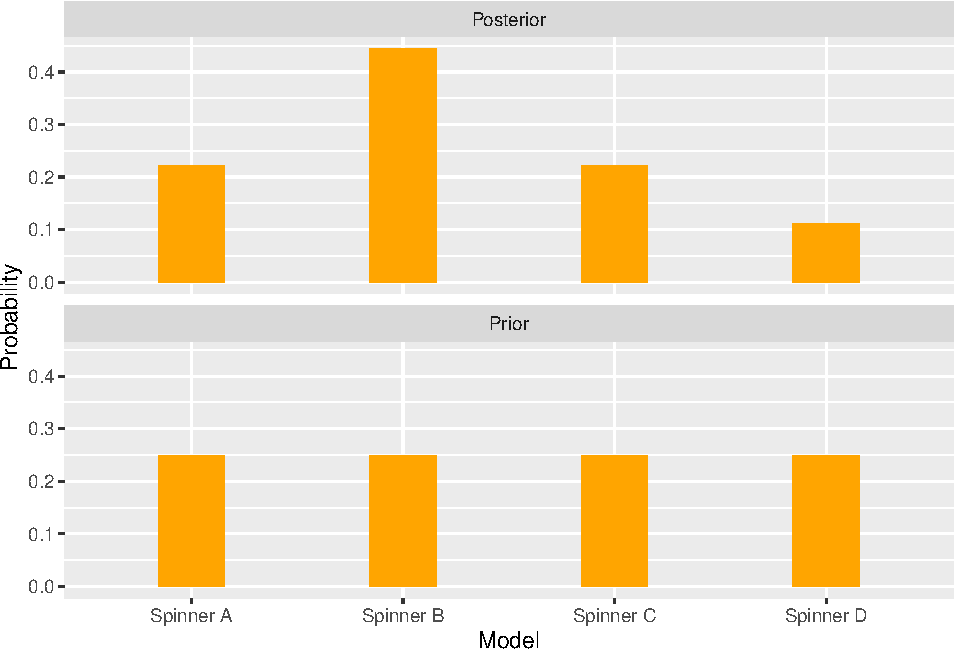
\includegraphics{bookdown-demo_files/figure-latex/unnamed-chunk-50-1.pdf}

\hypertarget{federalist-paper-study}{%
\chapter{Federalist Paper Study}\label{federalist-paper-study}}

\hypertarget{packages-for-this-example}{%
\section{Packages for this example}\label{packages-for-this-example}}

\begin{Shaded}
\begin{Highlighting}[]
\KeywordTok{library}\NormalTok{(tidyverse)}
\KeywordTok{library}\NormalTok{(brms)}
\KeywordTok{library}\NormalTok{(bayesplot)}
\KeywordTok{library}\NormalTok{(ProbBayes)}
\end{Highlighting}
\end{Shaded}

\hypertarget{federalist-paper-data}{%
\section{Federalist paper data}\label{federalist-paper-data}}

The data frame \texttt{federalist\_word\_study} contains frequency use of words for Federalist Papers written by either Alexander Hamilton or James Madison.

We'll focus on the frequencies of the word ``can'' in groups of 1000 words written by Hamilton

\begin{Shaded}
\begin{Highlighting}[]
\NormalTok{federalist_word_study }\OperatorTok\StringTok{ }
\StringTok{  }\KeywordTok{filter}\NormalTok{(word }\OperatorTok{==}\StringTok{ "can"}\NormalTok{,}
\NormalTok{         Authorship }\OperatorTok{==}\StringTok{ "Hamilton"}\NormalTok{) ->}\StringTok{ }\NormalTok{d}
\KeywordTok{head}\NormalTok{(d)}
\end{Highlighting}
\end{Shaded}

\begin{verbatim}
##                   Name Total word  N         Rate Authorship Disputed
## 65    Federalist No. 1  1622  can  3 0.0018495684   Hamilton       no
## 1526 Federalist No. 11  2511  can  5 0.0019912386   Hamilton       no
## 2437 Federalist No. 12  2171  can  2 0.0009212345   Hamilton       no
## 3125 Federalist No. 13   970  can  4 0.0041237113   Hamilton       no
## 4256 Federalist No. 15  3095  can 14 0.0045234249   Hamilton       no
## 5530 Federalist No. 16  2047  can  1 0.0004885198   Hamilton       no
\end{verbatim}

\hypertarget{the-poisson-sampling-model}{%
\section{The Poisson sampling model}\label{the-poisson-sampling-model}}

If \(y_i\) represents the count of ``can'' in the \(i\) group of words, we assume

\[
y_i  \sim Poisson(n_i \lambda / 1000), i = 1, ..., N
\]

where \(\lambda\) is the true rate of the word among 1000 words.

On log scale, the Poisson mean can be written

\[
\log E(y_i) = \log \lambda + \log(n_i / 1000)
\]
which can be fit as a generalized linear model with Poisson sampling, log link, intercept model with an offset of \(\log(n_i / 1000)\).

We complete this model by assigning the prior
\[
\log \lambda \sim N(0, 2)
\]

\hypertarget{fitting-the-model}{%
\section{Fitting the model}\label{fitting-the-model}}

We use the `\texttt{brm()} function with ``family = poisson'', specifying the offset ``N'', and specifying the prior by use of the ``prior'' argument.

\begin{Shaded}
\begin{Highlighting}[]
\NormalTok{fit <-}\StringTok{ }\KeywordTok{brm}\NormalTok{(}\DataTypeTok{data =}\NormalTok{ d, }\DataTypeTok{family =}\NormalTok{ poisson,}
\NormalTok{    N }\OperatorTok{~}\StringTok{ }\KeywordTok{offset}\NormalTok{(}\KeywordTok{log}\NormalTok{(Total }\OperatorTok{/}\StringTok{ }\DecValTok{1000}\NormalTok{)) }\OperatorTok{+}\StringTok{ }\DecValTok{1}\NormalTok{,}
    \DataTypeTok{prior =} \KeywordTok{c}\NormalTok{(}\KeywordTok{prior}\NormalTok{(}\KeywordTok{normal}\NormalTok{(}\DecValTok{0}\NormalTok{, }\DecValTok{2}\NormalTok{), }
                    \DataTypeTok{class =}\NormalTok{ Intercept)),}
              \DataTypeTok{refresh =} \DecValTok{0}
\NormalTok{    )}
\end{Highlighting}
\end{Shaded}

\begin{verbatim}
## Compiling Stan program...
\end{verbatim}

\begin{verbatim}
## recompiling to avoid crashing R session
\end{verbatim}

\begin{verbatim}
## Start sampling
\end{verbatim}

We display summaries of the posterior for \(\lambda\).

\begin{Shaded}
\begin{Highlighting}[]
\KeywordTok{summary}\NormalTok{(fit)}
\end{Highlighting}
\end{Shaded}

\begin{verbatim}
##  Family: poisson 
##   Links: mu = log 
## Formula: N ~ offset(log(Total/1000)) + 1 
##    Data: d (Number of observations: 49) 
## Samples: 4 chains, each with iter = 2000; warmup = 1000; thin = 1;
##          total post-warmup samples = 4000
## 
## Population-Level Effects: 
##           Estimate Est.Error l-95% CI u-95% CI Rhat Bulk_ESS Tail_ESS
## Intercept     0.97      0.06     0.86     1.08 1.00     1553     2145
## 
## Samples were drawn using sampling(NUTS). For each parameter, Bulk_ESS
## and Tail_ESS are effective sample size measures, and Rhat is the potential
## scale reduction factor on split chains (at convergence, Rhat = 1).
\end{verbatim}

We save \texttt{post} as a matrix of simulated draws.

\begin{Shaded}
\begin{Highlighting}[]
\NormalTok{post <-}\StringTok{ }\KeywordTok{posterior_samples}\NormalTok{(fit)}
\end{Highlighting}
\end{Shaded}

The function \texttt{mcmc\_areas()} displays a density estimate of the simulated draws and shows the location of a 50\% probability interval.

\begin{Shaded}
\begin{Highlighting}[]
\KeywordTok{mcmc_areas}\NormalTok{(post, }\DataTypeTok{pars =} \StringTok{"b_Intercept"}\NormalTok{)}
\end{Highlighting}
\end{Shaded}

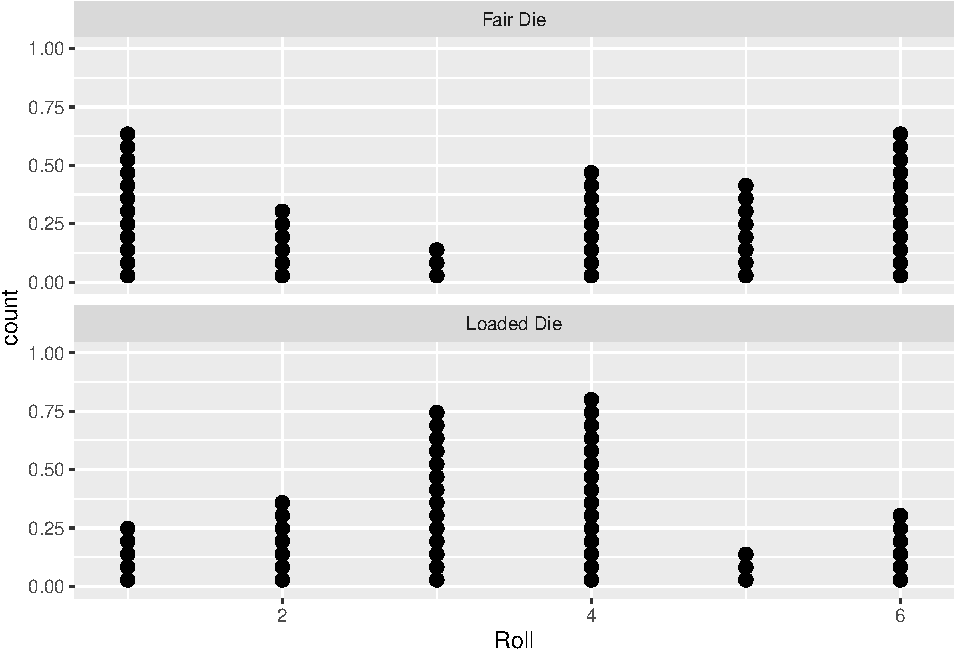
\includegraphics{bookdown-demo_files/figure-latex/unnamed-chunk-56-1.pdf}

\hypertarget{model-checking}{%
\section{Model checking}\label{model-checking}}

To check if the Poisson sampling model is appropriate we illustrate several posterior predictive checks.

Here we display density estimates for 10 replicated samples from the posterior predictive distribution of \(y\) and overlay the observed values as a dark line.

\begin{Shaded}
\begin{Highlighting}[]
\KeywordTok{pp_check}\NormalTok{(fit)}
\end{Highlighting}
\end{Shaded}

\begin{verbatim}
## Using 10 posterior samples for ppc type 'dens_overlay' by default.
\end{verbatim}

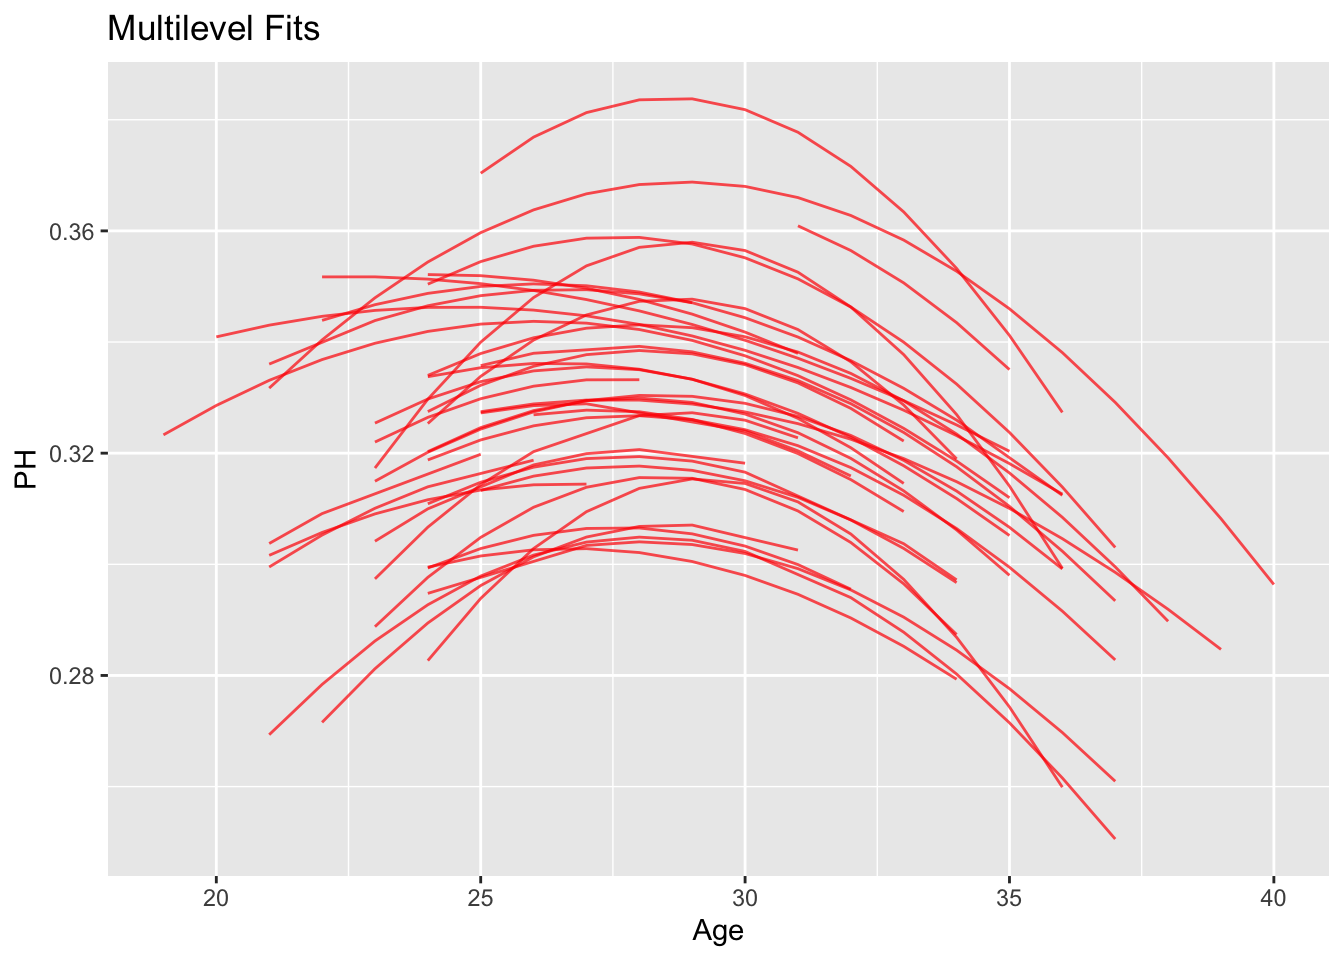
\includegraphics{bookdown-demo_files/figure-latex/unnamed-chunk-57-1.pdf}

Here we use \((\bar y, s_y)\) as a checking function. The scatterplot represents values of \((\bar y, s_y)\) from the posterior predictive distribution of replicated data, and the observed value of \((\bar y, s_y)\) is shown as a dot.

\begin{Shaded}
\begin{Highlighting}[]
\KeywordTok{pp_check}\NormalTok{(fit, }\DataTypeTok{type =} \StringTok{"stat_2d"}\NormalTok{)}
\end{Highlighting}
\end{Shaded}

\begin{verbatim}
## Using all posterior samples for ppc type 'stat_2d' by default.
\end{verbatim}

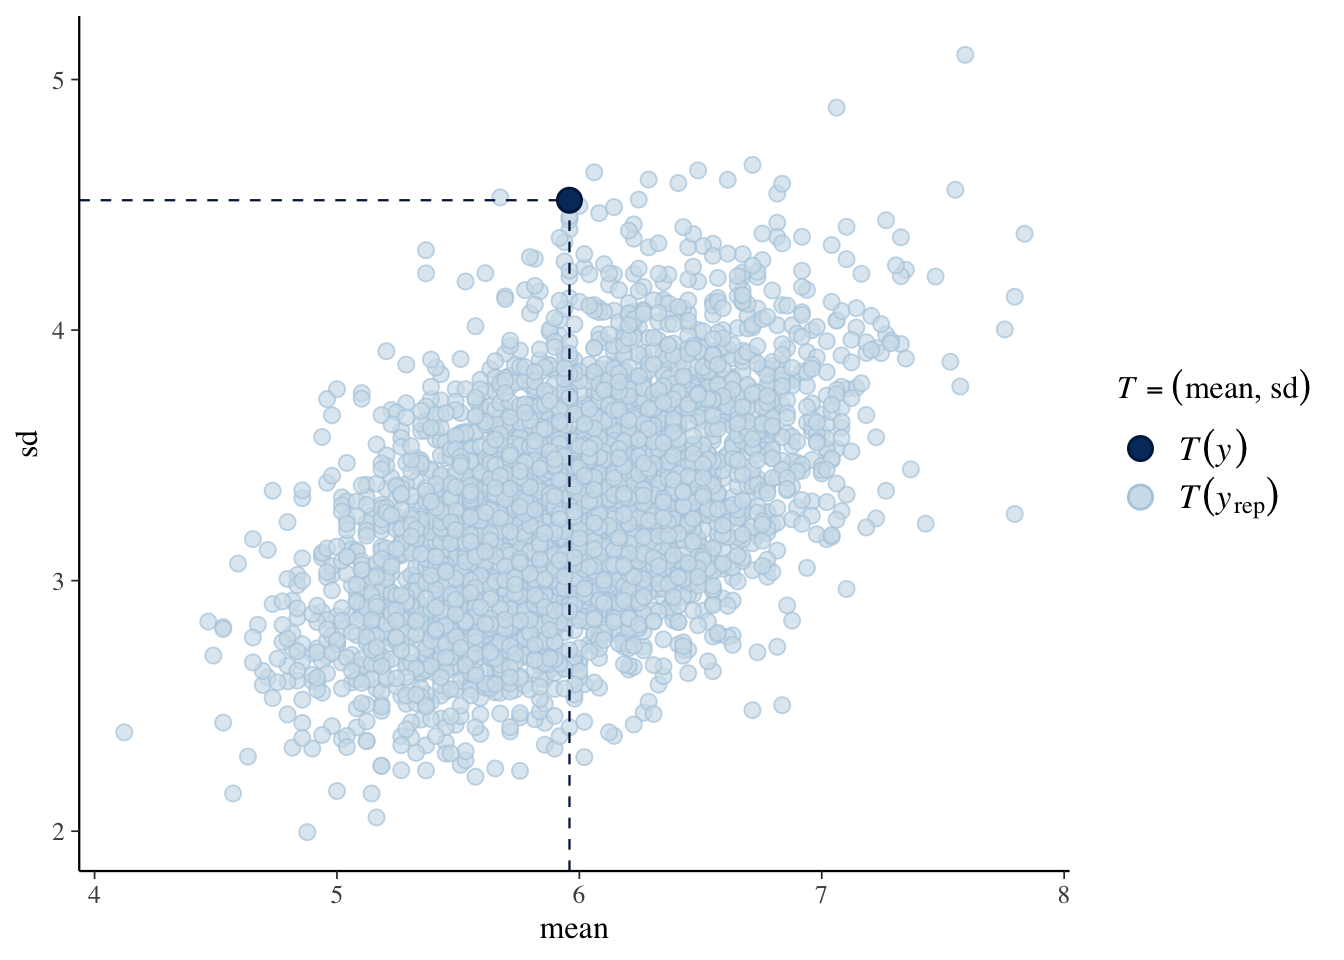
\includegraphics{bookdown-demo_files/figure-latex/unnamed-chunk-58-1.pdf}

The takeaway is that the observed data shows more variability than predicted from the Poisson sampling model.

\hypertarget{negative-binomial-sampling}{%
\section{Negative binomial sampling}\label{negative-binomial-sampling}}

One way to handle the extra variability is to assume that the \(y_i\) have a negative binomial distribution. (See the text for details.)

Here we outline the code for fitting this model.

We fit the model with the \texttt{brm()} function with the ``family = negbinomial'' option.

\begin{Shaded}
\begin{Highlighting}[]
\NormalTok{fit_nb <-}\StringTok{ }\KeywordTok{brm}\NormalTok{(}\DataTypeTok{data =}\NormalTok{ d, }\DataTypeTok{family =}\NormalTok{ negbinomial,}
\NormalTok{           N }\OperatorTok{~}\StringTok{ }\KeywordTok{offset}\NormalTok{(}\KeywordTok{log}\NormalTok{(Total }\OperatorTok{/}\StringTok{ }\DecValTok{1000}\NormalTok{)) }\OperatorTok{+}\StringTok{ }\DecValTok{1}\NormalTok{,}
           \DataTypeTok{refresh =} \DecValTok{0}\NormalTok{)}
\end{Highlighting}
\end{Shaded}

\begin{verbatim}
## Compiling Stan program...
\end{verbatim}

\begin{verbatim}
## Start sampling
\end{verbatim}

Here I can checking on the default priors used by brm:

\begin{Shaded}
\begin{Highlighting}[]
\KeywordTok{prior_summary}\NormalTok{(fit_nb)}
\end{Highlighting}
\end{Shaded}

\begin{verbatim}
##                    prior     class coef group resp dpar nlpar bound
## 1 student_t(3, 1.6, 2.5) Intercept                                 
## 2      gamma(0.01, 0.01)     shape
\end{verbatim}

Here are the posterior summaries.

\begin{Shaded}
\begin{Highlighting}[]
\KeywordTok{summary}\NormalTok{(fit_nb)}
\end{Highlighting}
\end{Shaded}

\begin{verbatim}
##  Family: negbinomial 
##   Links: mu = log; shape = identity 
## Formula: N ~ offset(log(Total/1000)) + 1 
##    Data: d (Number of observations: 49) 
## Samples: 4 chains, each with iter = 2000; warmup = 1000; thin = 1;
##          total post-warmup samples = 4000
## 
## Population-Level Effects: 
##           Estimate Est.Error l-95% CI u-95% CI Rhat Bulk_ESS Tail_ESS
## Intercept     1.00      0.10     0.80     1.19 1.00     2903     2668
## 
## Family Specific Parameters: 
##       Estimate Est.Error l-95% CI u-95% CI Rhat Bulk_ESS Tail_ESS
## shape     3.25      1.11     1.72     5.93 1.00     3023     2533
## 
## Samples were drawn using sampling(NUTS). For each parameter, Bulk_ESS
## and Tail_ESS are effective sample size measures, and Rhat is the potential
## scale reduction factor on split chains (at convergence, Rhat = 1).
\end{verbatim}

I save the posterior samples in the data frame \texttt{post}.

\begin{Shaded}
\begin{Highlighting}[]
\NormalTok{post <-}\StringTok{ }\KeywordTok{posterior_samples}\NormalTok{(fit)}
\end{Highlighting}
\end{Shaded}

I try the same posterior predictive checks as before. The message is that the negative binomial sampling model is a better fit to these data.

\begin{Shaded}
\begin{Highlighting}[]
\KeywordTok{pp_check}\NormalTok{(fit_nb)}
\end{Highlighting}
\end{Shaded}

\begin{verbatim}
## Using 10 posterior samples for ppc type 'dens_overlay' by default.
\end{verbatim}

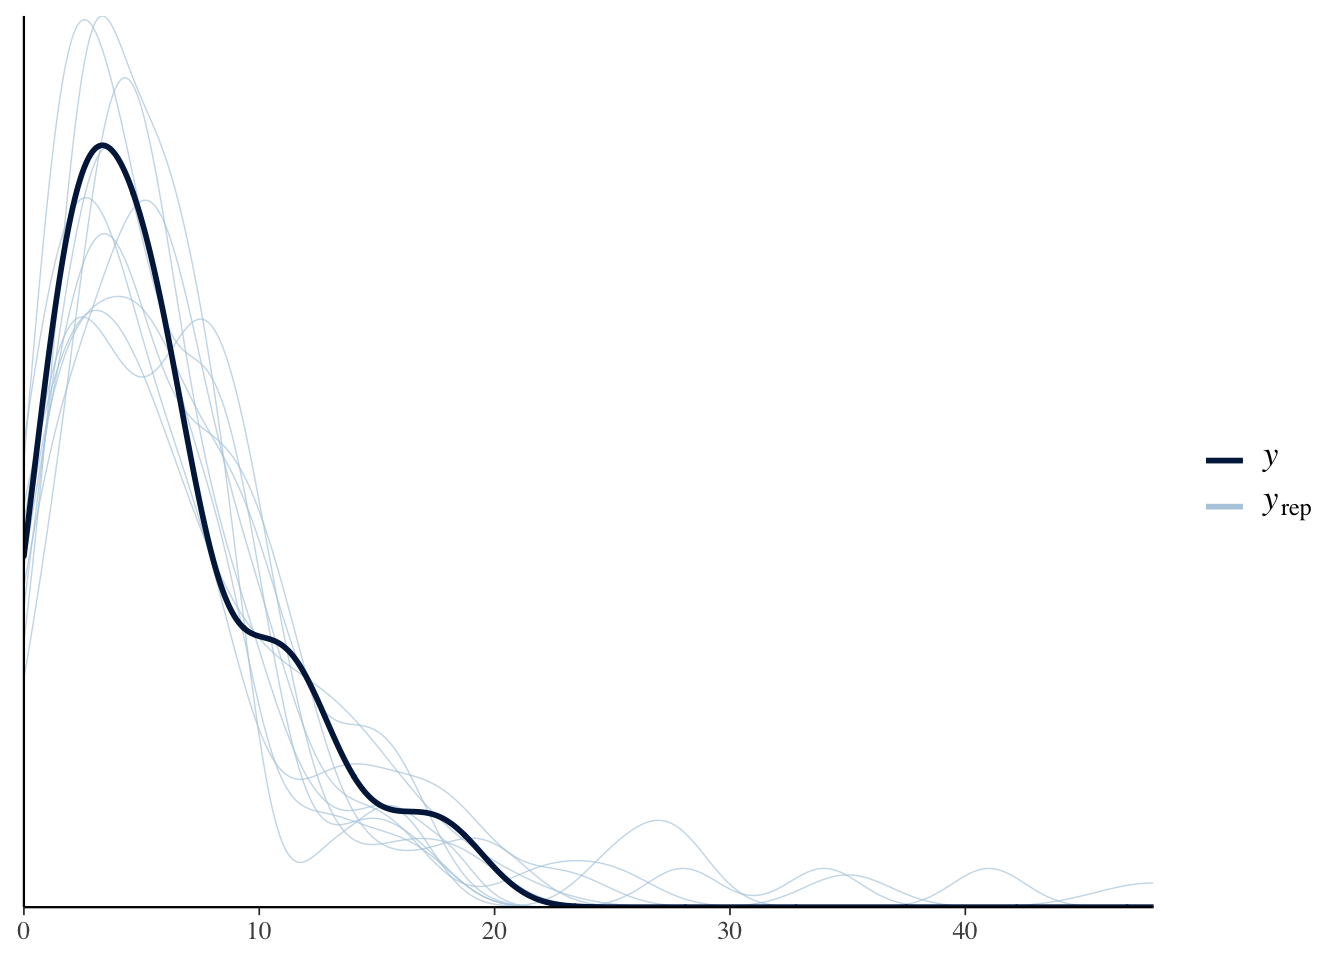
\includegraphics{bookdown-demo_files/figure-latex/unnamed-chunk-63-1.pdf}

\begin{Shaded}
\begin{Highlighting}[]
\KeywordTok{pp_check}\NormalTok{(fit_nb, }\DataTypeTok{type =} \StringTok{"stat_2d"}\NormalTok{)}
\end{Highlighting}
\end{Shaded}

\begin{verbatim}
## Using all posterior samples for ppc type 'stat_2d' by default.
\end{verbatim}

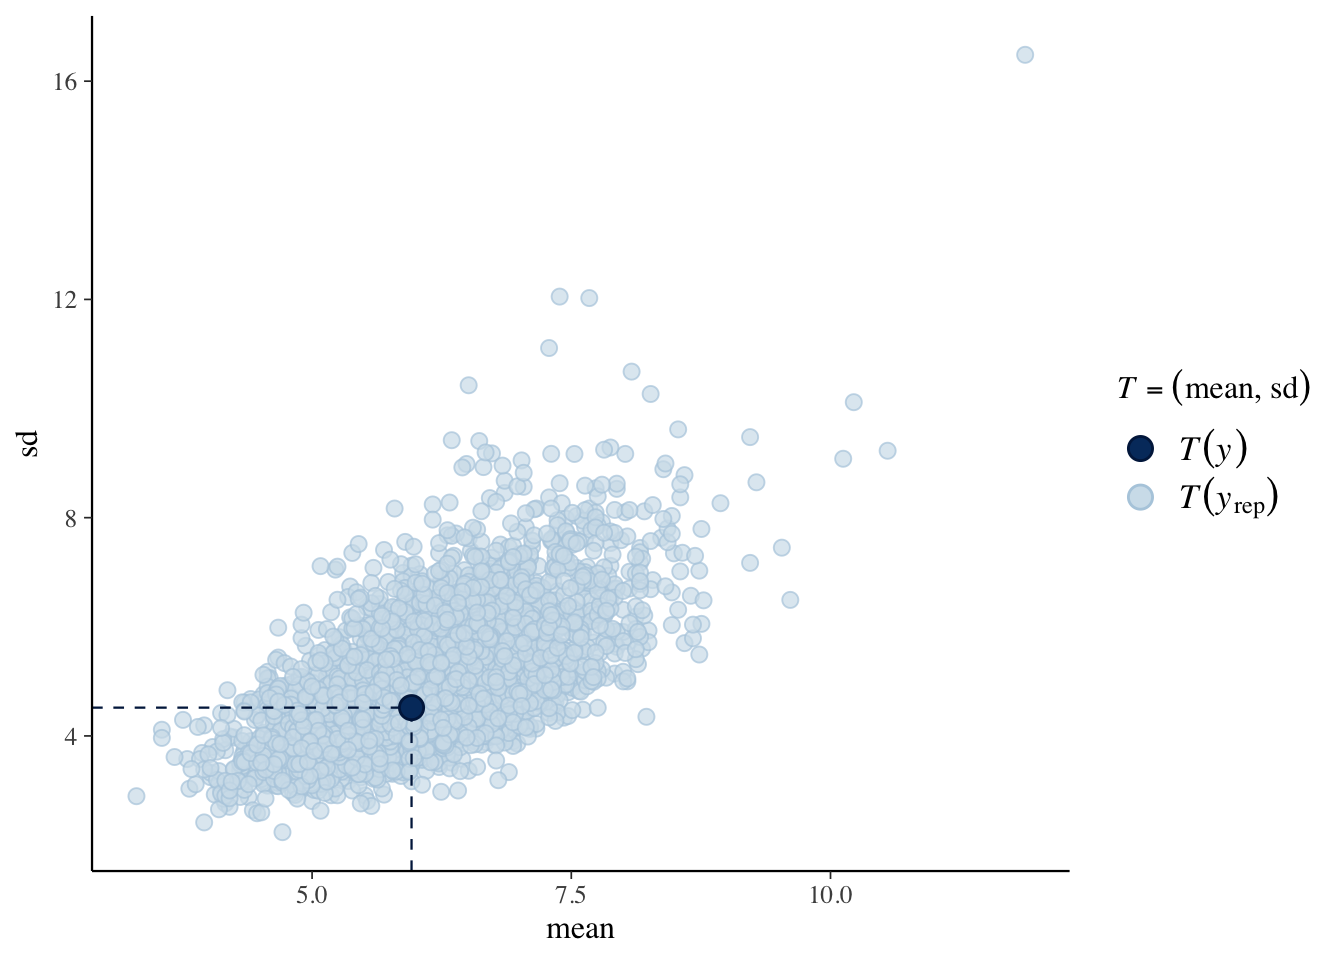
\includegraphics{bookdown-demo_files/figure-latex/unnamed-chunk-64-1.pdf}

\hypertarget{comparing-use-of-a-word}{%
\section{Comparing use of a word}\label{comparing-use-of-a-word}}

Next we compare Madison and Hamilton use of the word ``can''. The data frame \texttt{d2} contains only the word data for the essays that were known to be written by Hamilton or Madison.

\begin{Shaded}
\begin{Highlighting}[]
\NormalTok{federalist_word_study }\OperatorTok\StringTok{ }
\StringTok{  }\KeywordTok{filter}\NormalTok{(word }\OperatorTok{==}\StringTok{ "can"}\NormalTok{,}
\NormalTok{         Authorship }\OperatorTok\StringTok{ }\KeywordTok{c}\NormalTok{(}\StringTok{"Hamilton"}\NormalTok{, }\StringTok{"Madison"}\NormalTok{)) ->}\StringTok{ }\NormalTok{d2}
\end{Highlighting}
\end{Shaded}

Here I fit a regression model for the mean use of ``can'', where the one predictor is the categorical variable ``Authorship''.

\begin{Shaded}
\begin{Highlighting}[]
\NormalTok{fit_nb <-}\StringTok{ }\KeywordTok{brm}\NormalTok{(}\DataTypeTok{data =}\NormalTok{ d2, }\DataTypeTok{family =}\NormalTok{ negbinomial,}
\NormalTok{           N }\OperatorTok{~}\StringTok{ }\KeywordTok{offset}\NormalTok{(}\KeywordTok{log}\NormalTok{(Total }\OperatorTok{/}\StringTok{ }\DecValTok{1000}\NormalTok{)) }\OperatorTok{+}\StringTok{ }
\StringTok{          }\NormalTok{Authorship ,}
           \DataTypeTok{refresh =} \DecValTok{0}\NormalTok{)}
\end{Highlighting}
\end{Shaded}

\begin{verbatim}
## Compiling Stan program...
\end{verbatim}

\begin{verbatim}
## recompiling to avoid crashing R session
\end{verbatim}

\begin{verbatim}
## Start sampling
\end{verbatim}

By summarizing the fit, we can see if the two authors differ in their use of the word ``can'' in their writings.

\begin{Shaded}
\begin{Highlighting}[]
\KeywordTok{summary}\NormalTok{(fit_nb)}
\end{Highlighting}
\end{Shaded}

\begin{verbatim}
##  Family: negbinomial 
##   Links: mu = log; shape = identity 
## Formula: N ~ offset(log(Total/1000)) + Authorship 
##    Data: d2 (Number of observations: 74) 
## Samples: 4 chains, each with iter = 2000; warmup = 1000; thin = 1;
##          total post-warmup samples = 4000
## 
## Population-Level Effects: 
##                   Estimate Est.Error l-95% CI u-95% CI Rhat Bulk_ESS Tail_ESS
## Intercept             1.00      0.10     0.81     1.19 1.00     3762     2790
## AuthorshipMadison    -0.09      0.16    -0.41     0.23 1.00     3924     3136
## 
## Family Specific Parameters: 
##       Estimate Est.Error l-95% CI u-95% CI Rhat Bulk_ESS Tail_ESS
## shape     3.87      1.15     2.20     6.62 1.00     3949     2798
## 
## Samples were drawn using sampling(NUTS). For each parameter, Bulk_ESS
## and Tail_ESS are effective sample size measures, and Rhat is the potential
## scale reduction factor on split chains (at convergence, Rhat = 1).
\end{verbatim}

\hypertarget{multilevel-regression}{%
\chapter{Multilevel Regression}\label{multilevel-regression}}

\hypertarget{packages-for-example}{%
\section{Packages for example}\label{packages-for-example}}

\begin{Shaded}
\begin{Highlighting}[]
\KeywordTok{library}\NormalTok{(tidyverse)}
\KeywordTok{library}\NormalTok{(brms)}
\end{Highlighting}
\end{Shaded}

\hypertarget{some-baseball-data}{%
\section{Some baseball data}\label{some-baseball-data}}

The function \texttt{get\_onbase\_data()} function collects on-base data for all players born in the year 1977 who have had at least 1000 career plate appearances.

\begin{Shaded}
\begin{Highlighting}[]
\KeywordTok{source}\NormalTok{(}\StringTok{"get_onbase_data.R"}\NormalTok{)}
\NormalTok{d78 <-}\StringTok{ }\KeywordTok{get_onbase_data}\NormalTok{(}\DecValTok{1977}\NormalTok{, }\DecValTok{1000}\NormalTok{)}
\end{Highlighting}
\end{Shaded}

\begin{verbatim}
## `summarise()` ungrouping output (override with `.groups` argument)
\end{verbatim}

\begin{verbatim}
## `summarise()` regrouping output by 'playerID' (override with `.groups` argument)
\end{verbatim}

\begin{Shaded}
\begin{Highlighting}[]
\KeywordTok{unique}\NormalTok{(d78}\OperatorTok{$}\NormalTok{nameLast)}
\end{Highlighting}
\end{Shaded}

\begin{verbatim}
##  [1] "Beltran"    "Bergeron"   "Bigbie"     "Bloomquist" "Byrd"      
##  [6] "Caruso"     "Chavez"     "Davis"      "Ellis"      "Everett"   
## [11] "Fukudome"   "Furcal"     "Gerut"      "Gibbons"    "Gonzalez"  
## [16] "Hafner"     "Hinske"     "Hudson"     "Inge"       "Jimenez"   
## [21] "Jones"      "Monroe"     "Munson"     "Nieves"     "Overbay"   
## [26] "Pierre"     "Punto"      "Quinlan"    "Redman"     "Roberts"   
## [31] "Ross"       "Rowand"     "Sanchez"    "Thames"     "Tyner"     
## [36] "Wigginton"  "Wilkerson"  "Wilson"
\end{verbatim}

\hypertarget{quadratic-aging-model}{%
\section{Quadratic aging model}\label{quadratic-aging-model}}

Let \(y_{ij}\) denote the number of on-base events in \(n_{ij}\) opportunities (plate appearances) of the \(i\)th batter in the \(j\)th season. Assume that \(y_{ij}\) is binomial with sample size \(n_{ij}\) and probability of success \(p_{ij}\).

Assume that the on-base probabilities for the \(i\)th player satisfy the logistic model
\[
\log \left(\frac{p_{ij}}{1 - p_{ij}}\right) = \beta_{i0} + \beta_{i1} D_{ij} + \beta_{i2} D_{ij}^2
\]
where \(D_{ij} = x_{ij} - 30\), \(x_{ij}\) is the age of the \(i\)th player in the \(j\)th season.

\hypertarget{multilevel-prior}{%
\section{Multilevel Prior}\label{multilevel-prior}}

The \(i\)th player's trajectory is described by the regression vector \(\beta_i = (\beta_{i0}, \beta_{i1}, \beta_{i2})\). We place a two-stage prior on the trajectories \(\beta_1, ..., \beta_N\):

\begin{enumerate}
\def\labelenumi{\arabic{enumi}.}
\item
  \(\beta_1, ..., \beta_N\) are a sample from a multivariate normal density with mean \(\beta\) and variance-covariance matrix \(\Sigma\).
\item
  The second-stage parameters \(\beta\) and \(\Sigma\) are independent with weakly informative priors.
\end{enumerate}

\hypertarget{bayesian-fitting}{%
\section{Bayesian fitting}\label{bayesian-fitting}}

The fitting of this model is done using the \texttt{brm()} function.

\begin{Shaded}
\begin{Highlighting}[]
\NormalTok{fit <-}\StringTok{ }\KeywordTok{brm}\NormalTok{(OB }\OperatorTok{|}\StringTok{ }\KeywordTok{trials}\NormalTok{(PA) }\OperatorTok{~}\StringTok{ }\NormalTok{AgeD }\OperatorTok{+}\StringTok{ }\KeywordTok{I}\NormalTok{(AgeD }\OperatorTok{^}\StringTok{ }\DecValTok{2}\NormalTok{) }\OperatorTok{+}
\StringTok{             }\NormalTok{(AgeD }\OperatorTok{+}\StringTok{ }\KeywordTok{I}\NormalTok{(AgeD }\OperatorTok{^}\StringTok{  }\DecValTok{2}\NormalTok{) }\OperatorTok{|}\StringTok{ }\NormalTok{Player),}
           \DataTypeTok{data =} \KeywordTok{filter}\NormalTok{(d78, PA }\OperatorTok{>}\StringTok{ }\DecValTok{0}\NormalTok{),}
           \DataTypeTok{family =} \KeywordTok{binomial}\NormalTok{(}\StringTok{"logit"}\NormalTok{),}
           \DataTypeTok{refresh =} \DecValTok{0}\NormalTok{)}
\end{Highlighting}
\end{Shaded}

\begin{verbatim}
## Compiling Stan program...
\end{verbatim}

\begin{verbatim}
## recompiling to avoid crashing R session
\end{verbatim}

\begin{verbatim}
## Start sampling
\end{verbatim}

I find posterior means of the fitted trajectories for all players.

\begin{Shaded}
\begin{Highlighting}[]
\NormalTok{Player_Fits <-}\StringTok{ }\KeywordTok{coef}\NormalTok{(fit)}\OperatorTok{$}\NormalTok{Player[, }\StringTok{"Estimate"}\NormalTok{, ] }\OperatorTok\StringTok{ }
\StringTok{  }\KeywordTok{as.data.frame}\NormalTok{() }\OperatorTok\StringTok{ }
\StringTok{    }\KeywordTok{mutate}\NormalTok{(}\DataTypeTok{Player =} \DecValTok{1}\OperatorTok{:}\KeywordTok{max}\NormalTok{(d78}\OperatorTok{$}\NormalTok{Player))}
\end{Highlighting}
\end{Shaded}

\begin{Shaded}
\begin{Highlighting}[]
\NormalTok{d78 <-}\StringTok{ }\KeywordTok{inner_join}\NormalTok{(d78, Player_Fits, }\DataTypeTok{by =} \StringTok{"Player"}\NormalTok{)}
\end{Highlighting}
\end{Shaded}

\begin{Shaded}
\begin{Highlighting}[]
\NormalTok{d78 }\OperatorTok\StringTok{ }
\StringTok{  }\KeywordTok{mutate}\NormalTok{(}\DataTypeTok{PH =} \KeywordTok{plogis}\NormalTok{(Intercept }\OperatorTok{+}\StringTok{ }\NormalTok{AgeD.y }\OperatorTok{*}\StringTok{ }\NormalTok{AgeD.x }\OperatorTok{+}
\StringTok{                       }\NormalTok{IAgeDE2 }\OperatorTok{*}\StringTok{ }\NormalTok{AgeD.x }\OperatorTok{^}\StringTok{ }\DecValTok{2}\NormalTok{)) ->}\StringTok{ }\NormalTok{d78}
\end{Highlighting}
\end{Shaded}

\begin{Shaded}
\begin{Highlighting}[]
\KeywordTok{ggplot}\NormalTok{(d78, }\KeywordTok{aes}\NormalTok{(Age, PH, }\DataTypeTok{group =}\NormalTok{ Player)) }\OperatorTok{+}
\StringTok{  }\KeywordTok{geom_line}\NormalTok{(}\DataTypeTok{color =} \StringTok{"red"}\NormalTok{, }\DataTypeTok{alpha =} \FloatTok{0.7}\NormalTok{) }\OperatorTok{+}
\StringTok{  }\KeywordTok{ggtitle}\NormalTok{(}\StringTok{"Multilevel Fits"}\NormalTok{) }
\end{Highlighting}
\end{Shaded}

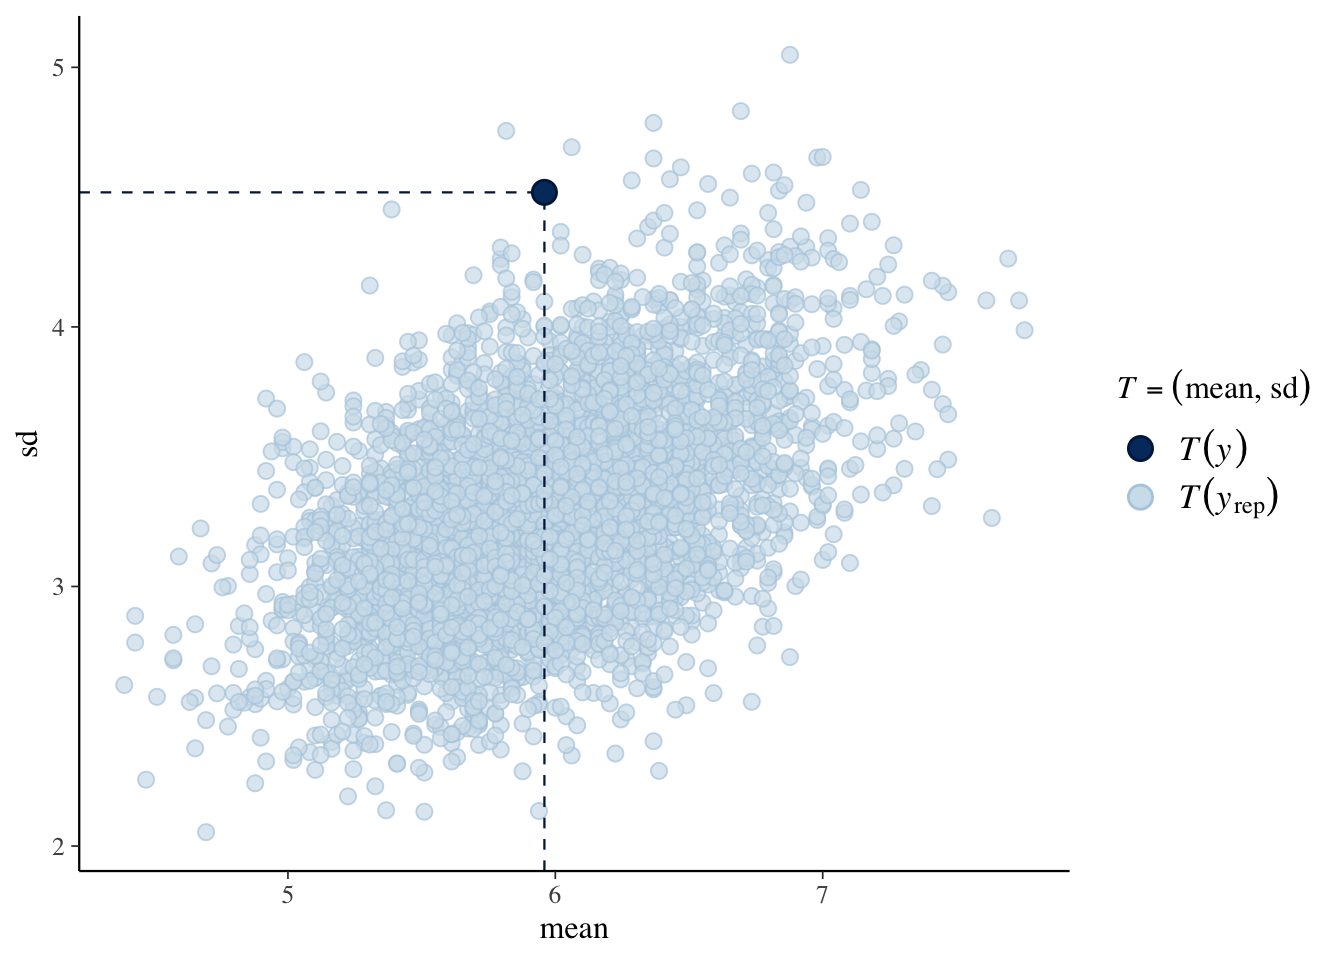
\includegraphics{bookdown-demo_files/figure-latex/unnamed-chunk-74-1.pdf}

For a given player, define the peak age
\[
Age_j = 30 - \frac{\beta_{j1}}{2 \beta_{j2}}.
\]
the age at which the player achieves peak performance.

The following graph shows the posterior distributions of the peak ages for all players.

\begin{Shaded}
\begin{Highlighting}[]
\NormalTok{d78  }\OperatorTok\StringTok{ }\KeywordTok{group_by}\NormalTok{(Player) }\OperatorTok\StringTok{ }
\StringTok{  }\KeywordTok{summarize}\NormalTok{(}\DataTypeTok{b0 =} \KeywordTok{first}\NormalTok{(Intercept),}
            \DataTypeTok{b1 =} \KeywordTok{first}\NormalTok{(AgeD.y),}
            \DataTypeTok{b2 =} \KeywordTok{first}\NormalTok{(IAgeDE2)) }\OperatorTok\StringTok{ }
\StringTok{  }\KeywordTok{mutate}\NormalTok{(}\DataTypeTok{MLM_Peak_Age =} \DecValTok{30} \OperatorTok{-}\StringTok{ }\NormalTok{b1 }\OperatorTok{/}\StringTok{ }\DecValTok{2} \OperatorTok{/}\StringTok{ }\NormalTok{b2)  }\OperatorTok\StringTok{ }
\StringTok{  }\KeywordTok{ggplot}\NormalTok{(}\KeywordTok{aes}\NormalTok{(MLM_Peak_Age)) }\OperatorTok{+}
\StringTok{  }\KeywordTok{geom_histogram}\NormalTok{(}\DataTypeTok{bins =} \DecValTok{12}\NormalTok{, }
                 \DataTypeTok{color =} \StringTok{"white"}\NormalTok{, }\DataTypeTok{fill =} \StringTok{"tan"}\NormalTok{) }\OperatorTok{+}
\StringTok{  }\KeywordTok{xlim}\NormalTok{(}\DecValTok{20}\NormalTok{, }\DecValTok{35}\NormalTok{)}
\end{Highlighting}
\end{Shaded}

\begin{verbatim}
## `summarise()` ungrouping output (override with `.groups` argument)
\end{verbatim}

\begin{verbatim}
## Warning: Removed 2 rows containing missing values (geom_bar).
\end{verbatim}

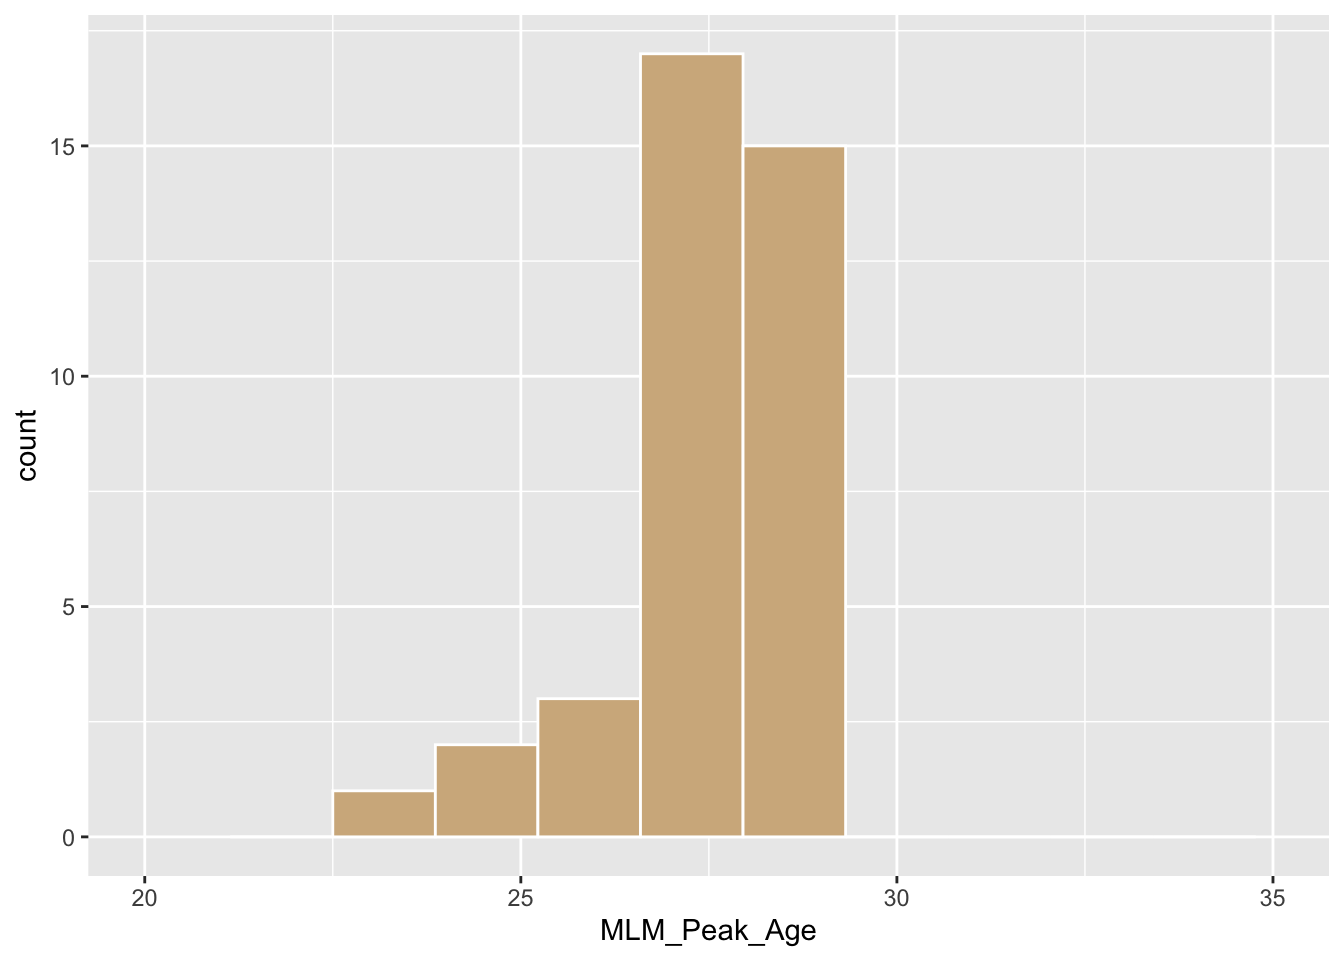
\includegraphics{bookdown-demo_files/figure-latex/unnamed-chunk-75-1.pdf}

  \bibliography{book.bib,packages.bib}

\end{document}
